\documentclass{newlayout}
%Bitte hier den enstprechenden Ort einsetzen z.B. Braunschweig und die Akademienummer
\Akademie{Rossleben}{2017}{5}

\usepackage[ngerman,english]{babel}
\usepackage{misc}
\usepackage{multicol}
\usepackage{booktabs}

\usepackage{color}% für Farben im allgemeinen
\usepackage{colortbl}

\usepackage{url}
\usepackage{breakurl}

\usepackage{units}

% hinzugef?gt, um Fehler 'pdfTeX error (font expansion): auto expansion is only possible with scalable' zu vermeiden
%\usepackage{lmodern}
\setkomafont{descriptionlabel}{\normalfont\bfseries}
\addtokomafont{paragraph}{\normalfont}
\usepackage{footnote}
\usepackage[flushmargin,hang,ragged]{footmisc}
\deffootnote{1em}{1em}{%
\textsuperscript{\thefootnotemark\ }
}

%\usepackage{amsmath}%wird automatisch durch newlayout.cls geladen
\usepackage{amsfonts}

%%%%%Mathe-Definitionen
\newtheorem{Def}{Definition}
\newtheorem{Sat}{Satz}
\newtheorem{Bew}{Beweis}

\setlength\abovedisplayshortskip{0pt}
\setlength\belowdisplayshortskip{0pt}
\setlength\abovedisplayskip{3pt}
\setlength\belowdisplayskip{3pt}
%%%%Ende Mathe-Definitionen

\begin{document}

 %   \input{titel}
 \setcounter{page}{3}

\setcounter{tocdepth}{1}
 \tableofcontents

   \setcounter{secnumdepth}{1}


\setcounter{page}{7}
\setcounter{chapter}{0}

%Angabe, bis zu welcher Stufe die sections im Text nummeriert werden sollen.
      \settocdepth{2}

\graphicspath{ {./pics/} }


\course{1}{Die Farbe Blau}%%% 
\begin{coursetitle}
  \centerline{Die Farbe Blau} 
  \bigskip
  %\Large \centerline{Kursuntertitel eingeben}
  \bigskip
 %\includegraphics[width=.9\textwidth]{kurslogo.png}
 \label{fig:meinbild}
  \bigskip
\end{coursetitle}


%\section{Gasentladung}

\section{Licht und Farbe}

author: Ailin Sigel, Selin Güler

Um zu verstehen, wie Farbigkeit zustande kommt, sollte man zunächst erwähnen, dass Licht einen Wellencharakter und spezifische Welleneigenschaften hat. Die Lichtwellen lassen sich nach ihrer Länge und  enthaltenden Energie im Spektrum elektromagnetischer Wellen einordnen.

Menschen können nur einen kleinen Teil des elektromagnetischen Spektrums wahrnehmen, den so genannten sichtbaren Bereich (siehe Abbildung \ref{dsafigure:beispiel}). Dieser erstreckt sich über Wellenlängen von 380 nm bis 780 nm und beinhaltet die Farben Violett, Blau, Grün, Gelb, Orange und Rot. 

\begin{dsafigure}
 \centering
 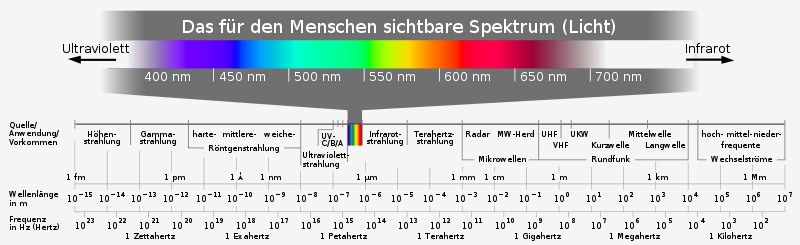
\includegraphics[width=\columnwidth]{pics/elektromagnetisches_Spektrum.png}
 \caption{Elektromagnetisches Spektrum mit dem für den Menschen sichtbaren Bereich des Spektrums.  \cite{elektromagnetisches_Spektrum}}
 \label{dsafigure:beispiel}
\end{dsafigure}

Das Sonnenlicht enthält alle Farben dieses Farbspektrums und erscheint deshalb weiß. Wenn die Lichtquelle ausgeschaltet ist, sehen wir schwarz, da kein Licht ausgestrahlt wird. Wird bei diesem additiven Farbsystem zum Beispiel das Licht von einer blauen und einer roten Lampe addiert, entsteht die Farbe Magenta (siehe Abbildung \ref{dsafigure:farbkreis}). Im Gegensatz dazu wird das Licht einer Lichtquelle (zum Beispiel der Sonne) von allen Gegenständen reflektiert. 
Bei diesem substraktivem Farbsystem ergibt sich die Farbe Schwarz aus der gemeinsamen Absorption von Wellenlängen aller Farben (siehe Abbildung \ref{dsafigure:farbkreis}).

Den Zusammenhang zwischen der Wellenlänge und der Energie lässt sich mit folgender Formel erklären:

\begin{equation}
E = \frac{h \cdot c}{\lambda} 
= h \cdot \nu
\end{equation}

$E$ beschreibt die Energie des Photons, $h$ das Plancksches Wirkungsquantum, $c$ die Lichtgeschwindigkeit, $\lambda$ die Wellenlänge, und $\nu$ die Frequenz.
Bei einer höheren Energie hat das Licht eine höhere Frequenz und dementsprechend ist die Wellenlänge kürzer. Umgekehrt bedeutet es auch, dass das Licht bei einer niedrigeren Energie eine niedrigere Frequenz und somit auch eine längere Wellenlänge hat.

\begin{dsafigure}
 \centering
 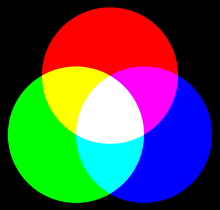
\includegraphics[width=0.45\columnwidth]{Additives_Farbsystem.png}
  \hfill
 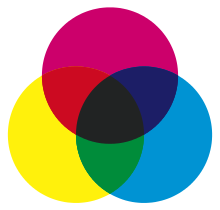
\includegraphics[width=0.45\columnwidth]{Substraktives_Farbsystem.png}
 \caption{Additives Farbsystem (links)\cite{Additives_Farbsystem} und Substraktives Farbsystem (rechts)\cite{Subtraktives_Farbsystem}}
 \label{dsafigure:farbkreis}
\end{dsafigure}


Der Zusammenhang zwischen Licht und Farbigkeit liegt an der Absorption und Reflexion von Licht. Dieses fällt durch die Pupille ins Auge und trifft dort auf die Netzhaut, die wiederum aus Stäbchen und Zapfen besteht. Die Stäbchen sind bei schwachen Lichteinfall aktiv und wir können damit nur schwarz-weiß sehen. Die Zapfen befinden sich im Zentrum der Netzhaut und sind besonders bei hohem Lichteinfall aktiv. Es gibt drei unterschiedliche Arten von Zapfen, die s-Zapfen, die als blaue Rezeptoren fungieren, die m-Zapfen, die als grüne Rezeptoren fungieren und die l-Zapfen, die als rote Rezeptoren fungieren. Jeder der Zapfen hat sein Maximum bei einer anderen Wellenlänge und zusammen decken sie somit den sichtbaren Bereich des elektromagnetischen Spektrums ab. 
Bei Anregung der Zapfen durch Licht, leiten sie einen Reiz an das Gehirn weiter. Durch die Kombination der verschiedenen angeregten Zapfen sehen wir Farbe.
Betrachten wir einen blauen Stift, der von der Sonne angeleuchtet wird, dann erscheint er uns blau. Was wir allerdings nicht sehen ist, dass die Elektronen im Stift vom Licht angeregt werden und vom Grundzustand in ein höheres Energieniveau angehoben werden (siehe Abbildung \ref{dsafigure:Grundzustand} ). Da dieser Zustand sehr instabil ist, fällt das Elektron wieder in seinen Grundzustand zurück. Dabei erfolgt die so genannten Relaxation über Schwingungen des Systems und es entsteht Wärme (siehe Abbildung \ref{dsafigure:Grundzustand}). Dass wir den Stift als blau wahrnehmen liegt daran, dass er die Komplementärfarbe zu Blau, also Gelb, absorbiert. Durch das fehlen der gelben Wellenlänge im reflektiertem Licht des Stiftes, interpretiert das Gehirn ihn als blau (siehe Abbildung \ref{dsafigure:farbkreis}, additives Farbsystem).
Wird blaues Licht durch einen Prozess emittiert, wird dieses ebenfalls als blau wahrgenommen.


\begin{dsafigure}
 \centering
 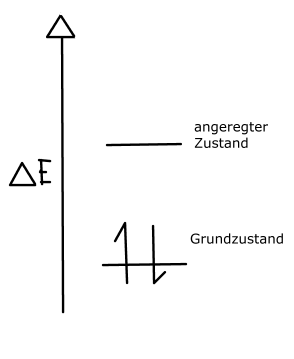
\includegraphics[width=0.45\columnwidth]{Grundzustand.png}
   \hfill
   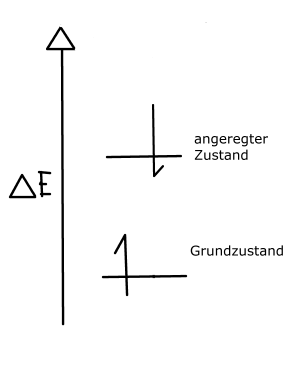
\includegraphics[width=0.45\columnwidth]{angeregter_Zustand.png}
 \caption{Elektronen im Grundzustand (links) und im angeregten Zustand (rechts)}
 \label{dsafigure:Grundzustand}
\end{dsafigure}


%\section{Atomorbitale}
\authors{Johannes Wörsdörfer, Ali Serour}

Atomorbitale sind Einteilchen-Wellenfunktionen. Sie sind Lösungen der Schrödingergleichung für das Wasserstoffatom beziehungsweise für Ionen mit nur einem Elektron. Die Aufenthaltswahrscheinlichkeitsdichte der Elektronen ergibt sich aus dem Betragsquadrat der Funktion. Demnach erwies sich die Vorstellung, dass sich die Elektronen eines Atoms in Schalen bewegen, als unvollständig. Darauf wird im Kapitel Schrödingergleichung  näher eingegangen.

Atomorbitale werden mithilfe von vier Quantenzahlen klassifiziert. Die Hauptquantenzahl $n$ definiert das Energieniveau des Elektrons. Die Nebenquantenzahl $l$ bestimmt die Geometrie der Orbitale. Sie kann die Werte $l = 0, 1, ..., n-1$ annehmen. Die magnetische Quantenzahl $m$ beschreibt den Drehimpuls eines Elektrons und somit die Ausrichtung des Orbitals im Raum. Es gibt die magnetischen Quantenzahlen $m = -l,...,l$. Die vierte Zahl ist die Spinquantenzahl $s$. Diese kann die Werte $s = -\frac{1}{2}, \frac{1}{2}$ annehmen \cite{Riedel07}. 

Um größere Atome beschreiben zu können, bedienen wir uns einer Näherung: Wir konstruieren die Vielteilchenwellenfunktion mithilfe von Einteilchenwellenfunktionen, die mit Elektronen besetzt werden. Dabei müssen drei Regeln beachtet werden: Das Aufbauprinzip besagt, dass zuerst alle energieärmeren Niveaus besetzt werden, bevor das darüber liegende Orbital besetzt wird. Die Hundsche Regel schreibt vor, dass bei einer Entartung eines Orbitals zuerst alle Orbitale mit gleicher Nebenquantenzahl $l$ mit dem gleichen Spin besetzt werden. Das Pauli-Prinzip gibt an, dass ein Orbital nur mit zwei Elektronen mit entgegengesetztem Spin besetzt werden kann, da es nicht zwei Elektronen mit exakt den selben Quantenzahlen innerhalb eines Atoms geben darf.

Im Folgenden wird dieses Modell anhand des Kohlenstoffatoms mithilfe eines Energieniveaudiagramms illustriert (siehe Abb. \ref{fig:Energieniveaudiagramm}). Kohlenstoff hat die Ordnungszahl 6. Es besitzt somit 6 Elektronen. Die Orbitale werden von unten nach oben mit Elektronen aufgefüllt, da Elektronen die energetisch günstigste Anordnung anstreben.  Die Elektronenkonfiguration für Kohlenstoff lautet $1s^{2} 2s^{2} 2p^{2}$. Die vorderen Zahlen geben die Hauptquantenzahl an. Der Buchstabe bezeichnet die Nebenquantenzahl der Orbitale mit $s$ für $l = 0$ und $p$ für $l=1$ und der Exponent definiert die Anzahl der Elektronen im jeweiligen Orbital.

\begin{dsafigure}
 \centering
 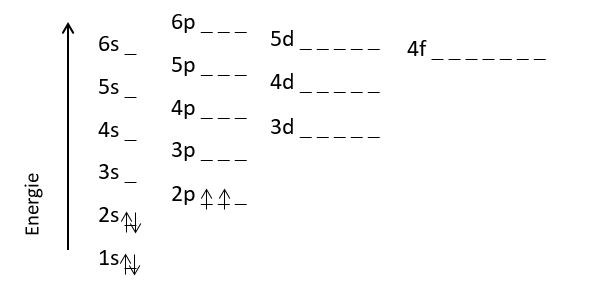
\includegraphics[width=8cm]{Energieniveaudiagramm.png}
 \caption{Die Besetzung der Orbitale nach dem Aufbauprinzip, der Hunschen Regel und dem Pauli-Prinzip ist anhand des Kohlenstoffatoms mithilfe eines Energieniveaudiagramms illustriert.}
 \label{fig:Energieniveaudiagramm}
\end{dsafigure}

Zum besseren Verständnis betrachten wir nun die räumliche Gestalt der Orbitale. Das s-Orbital hat die Form einer Kugel (siehe Abb. \ref{fig:s}). Die Nebenquantenzahl beträgt $0$. Außerdem hat es keine Knotenebene. Das p-Orbital hat die Nebenquantenzahl 1. Es gibt genau drei Magnetquantenzahlen $m = -1, 0, 1$. Das Orbital mit der magnetischen Quantenzahl $0$ hat die Form einer Hantel entlang der $z$-Achse. Es wir auch als $p_{z}$ bezeichnet (siehe Abb. \ref{fig:pz}). Aus den Zuständen $m = -1$ und $1$ werden die Linearkombinationen $p_{x} = \frac{1}{\sqrt{2}} (p_{+1} - p_{-1})$ (siehe Abb. \ref{fig:px}) und $p_{y} = \frac{i}{\sqrt{2}}(p_{+1}+p_{-1})$ (siehe Abb. \ref{fig:py} ) gebildet. Gleiches lässt sich auch auf d-Orbitale übertragen (siehe Abb. \ref{fig:dz2} - \ref{fig:dyz}).

\begin{dsafigure}
 \centering
 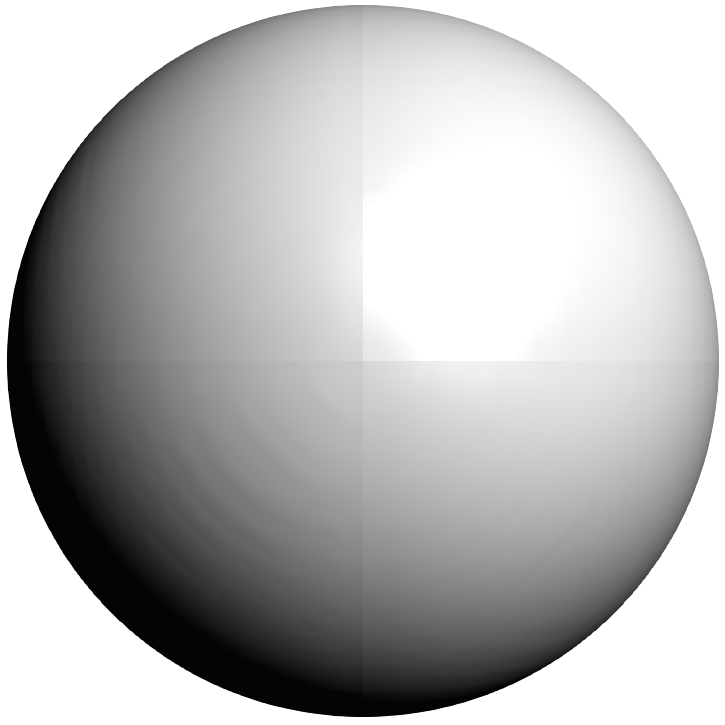
\includegraphics[width=8cm]{s.png}
 \caption{Darstellung eines s-Orbitals \cite{ADF2017authors}.}
 \label{fig:s}
\end{dsafigure}

\begin{dsafigure}
 \centering
 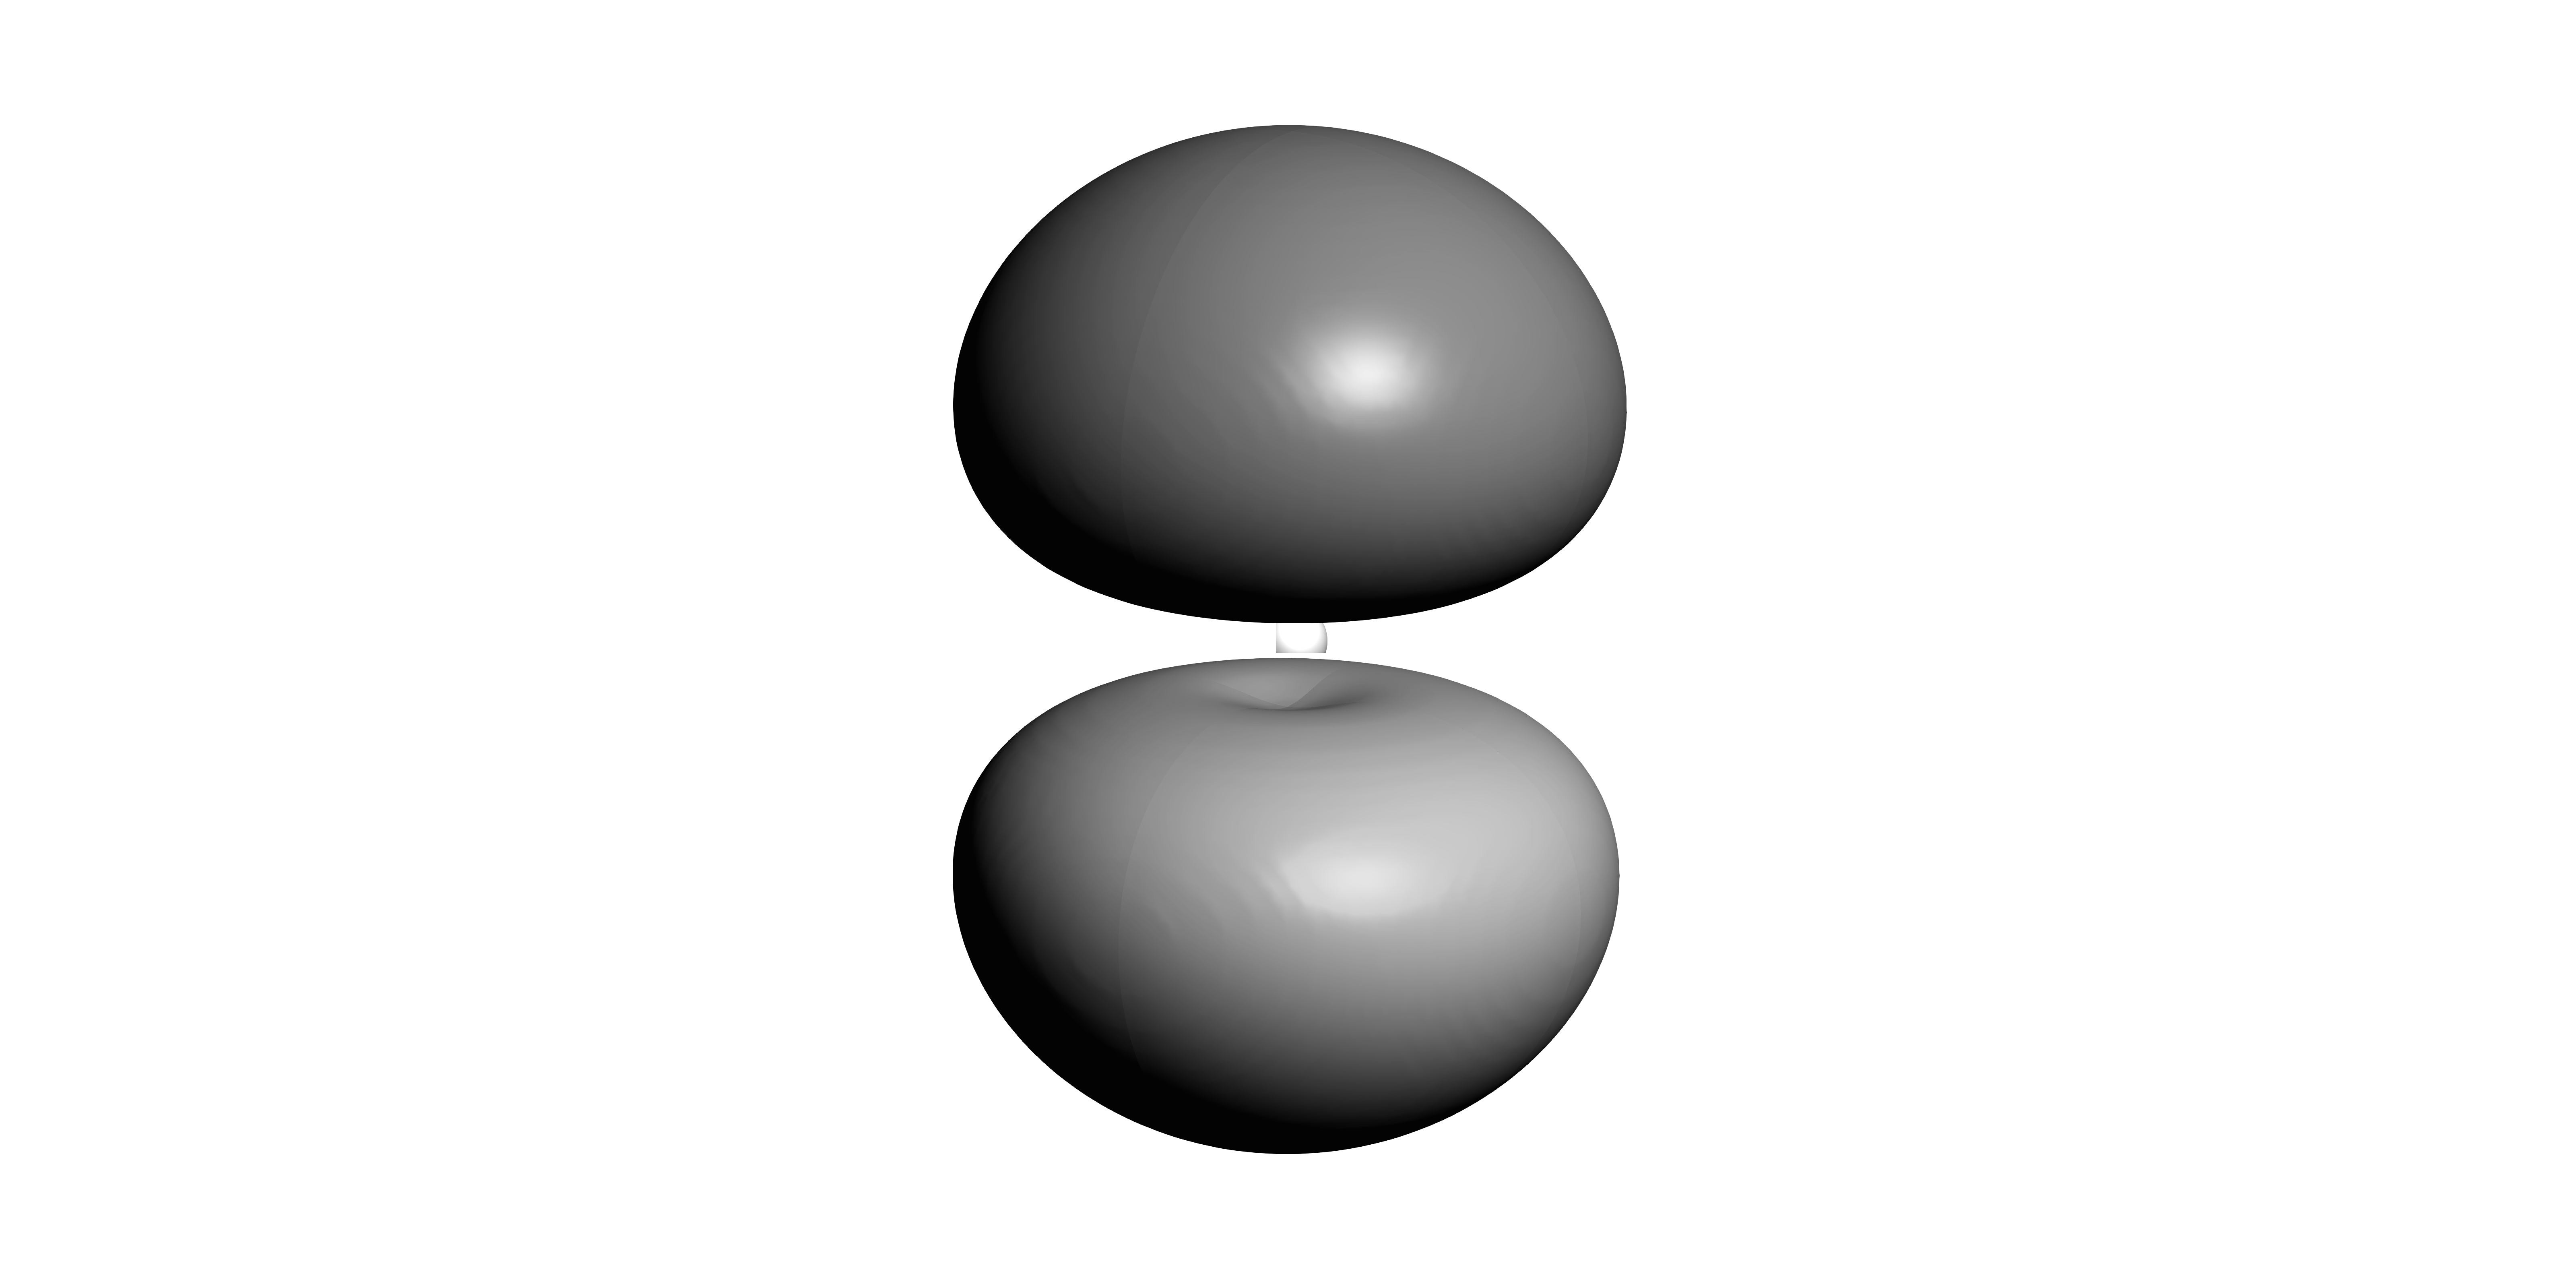
\includegraphics[width=8cm]{pz.png}
 \caption{Darstellung eines p$_{z}$-Orbitals \cite{ADF2017authors}.}
 \label{fig:pz}
\end{dsafigure}

\begin{dsafigure}
 \centering
 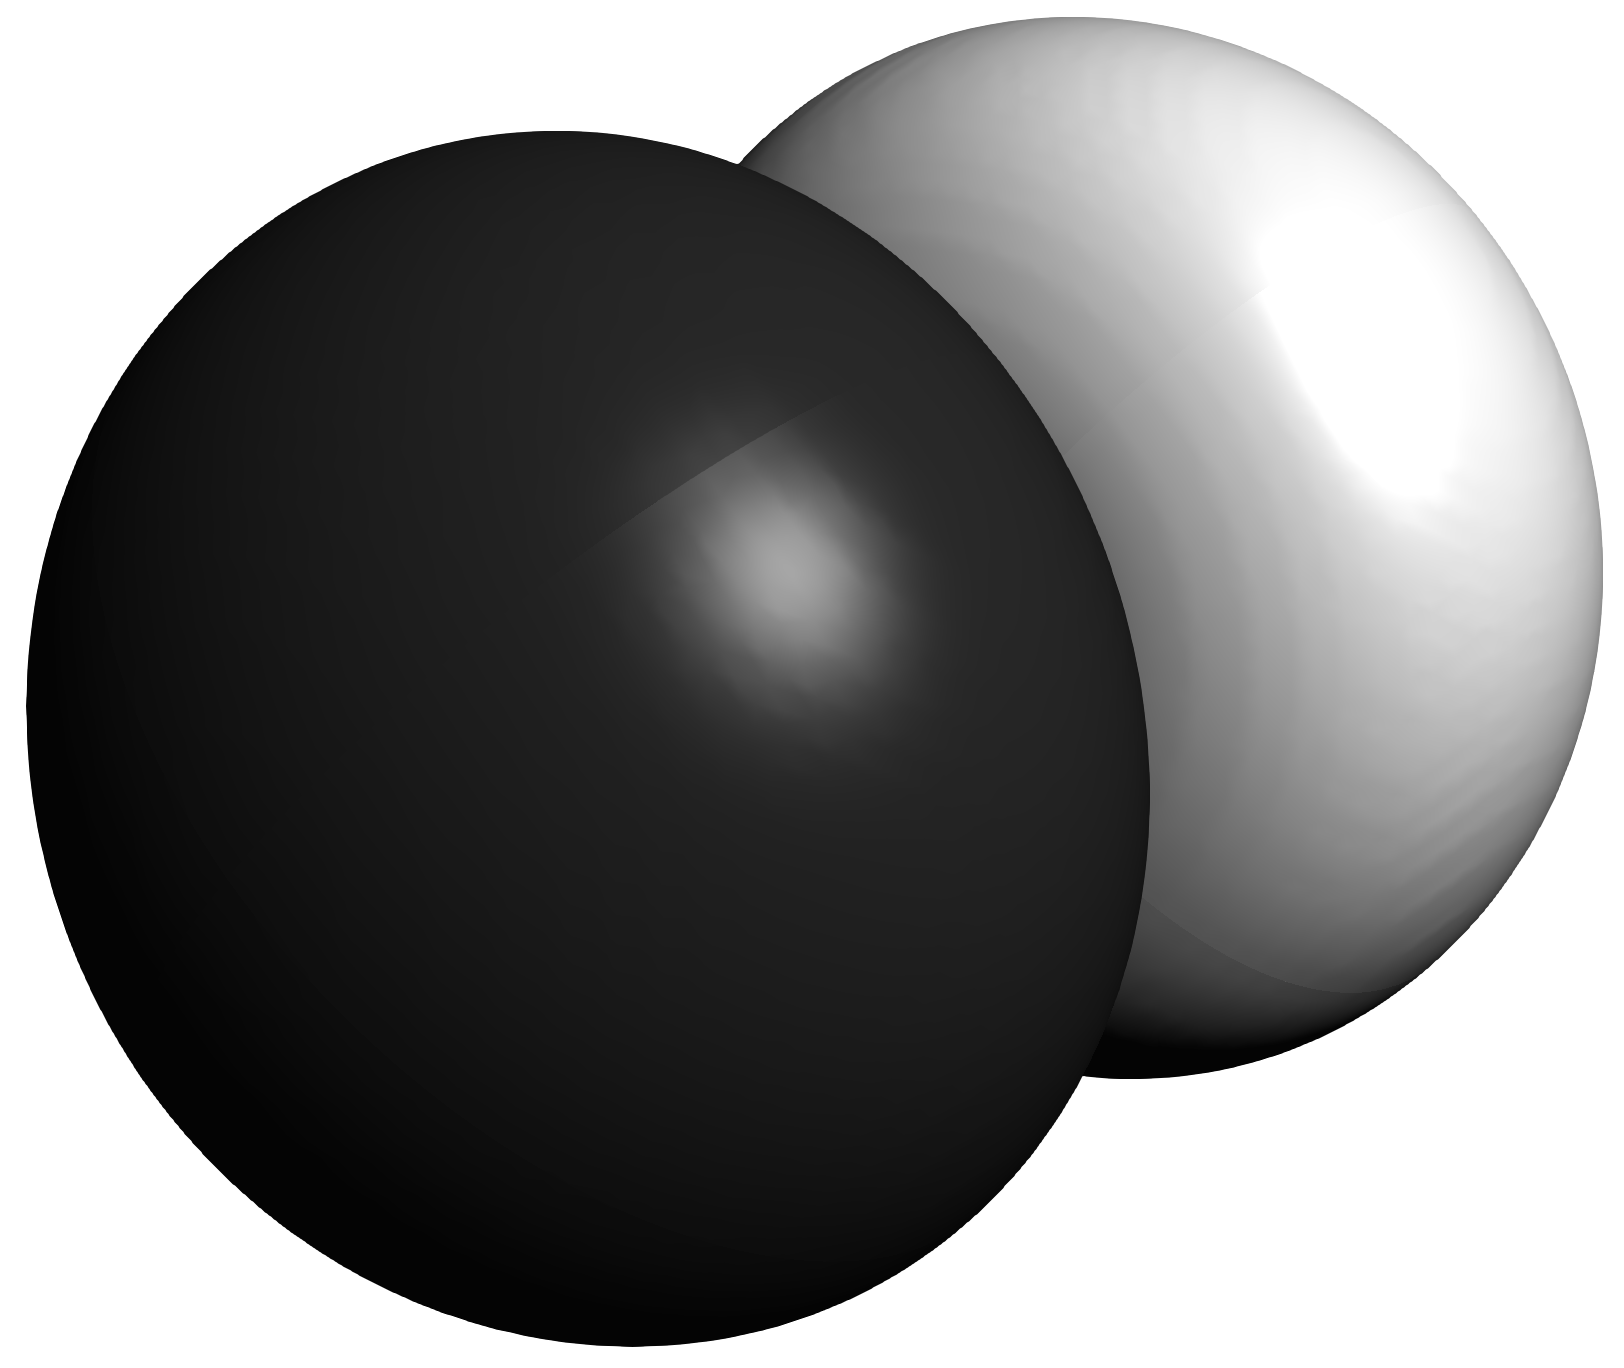
\includegraphics[width=8cm]{px.png}
 \caption{Darstellung eines p$_{x}$-Orbitals \cite{ADF2017authors}.}
 \label{fig:px}
\end{dsafigure}

\begin{dsafigure}
 \centering
 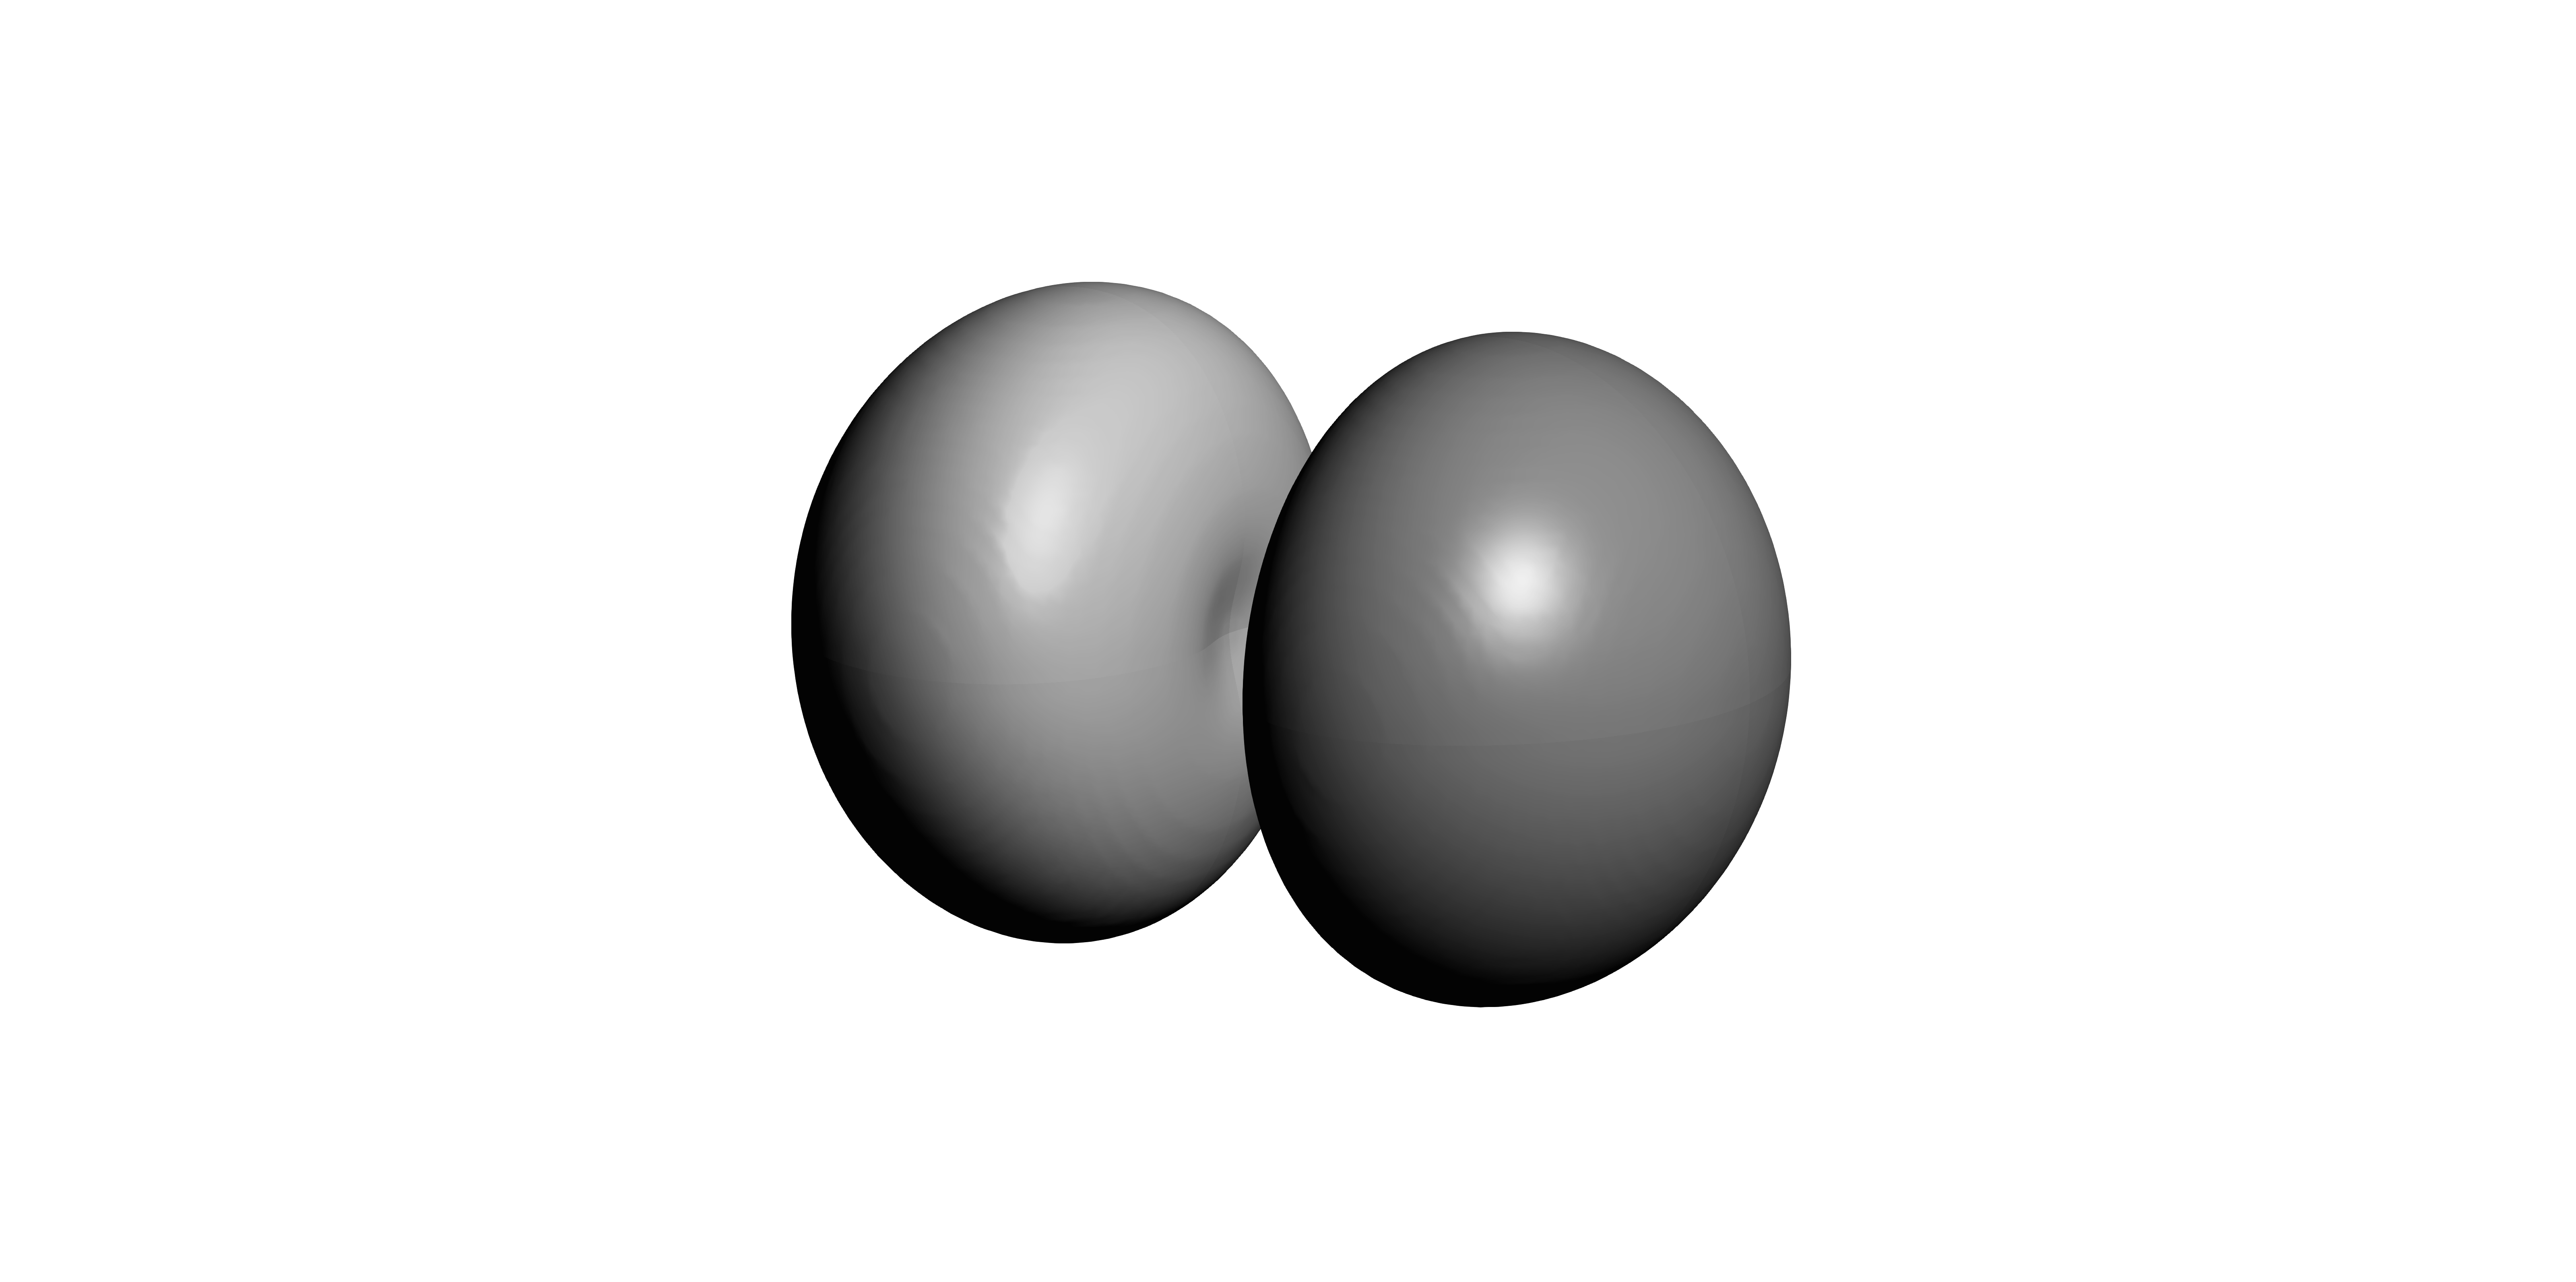
\includegraphics[width=8cm]{py.png}
 \caption{Darstellung eines p$_{y}$-Orbitals \cite{ADF2017authors}.}
 \label{fig:py}
\end{dsafigure}

\begin{dsafigure}
 \centering
 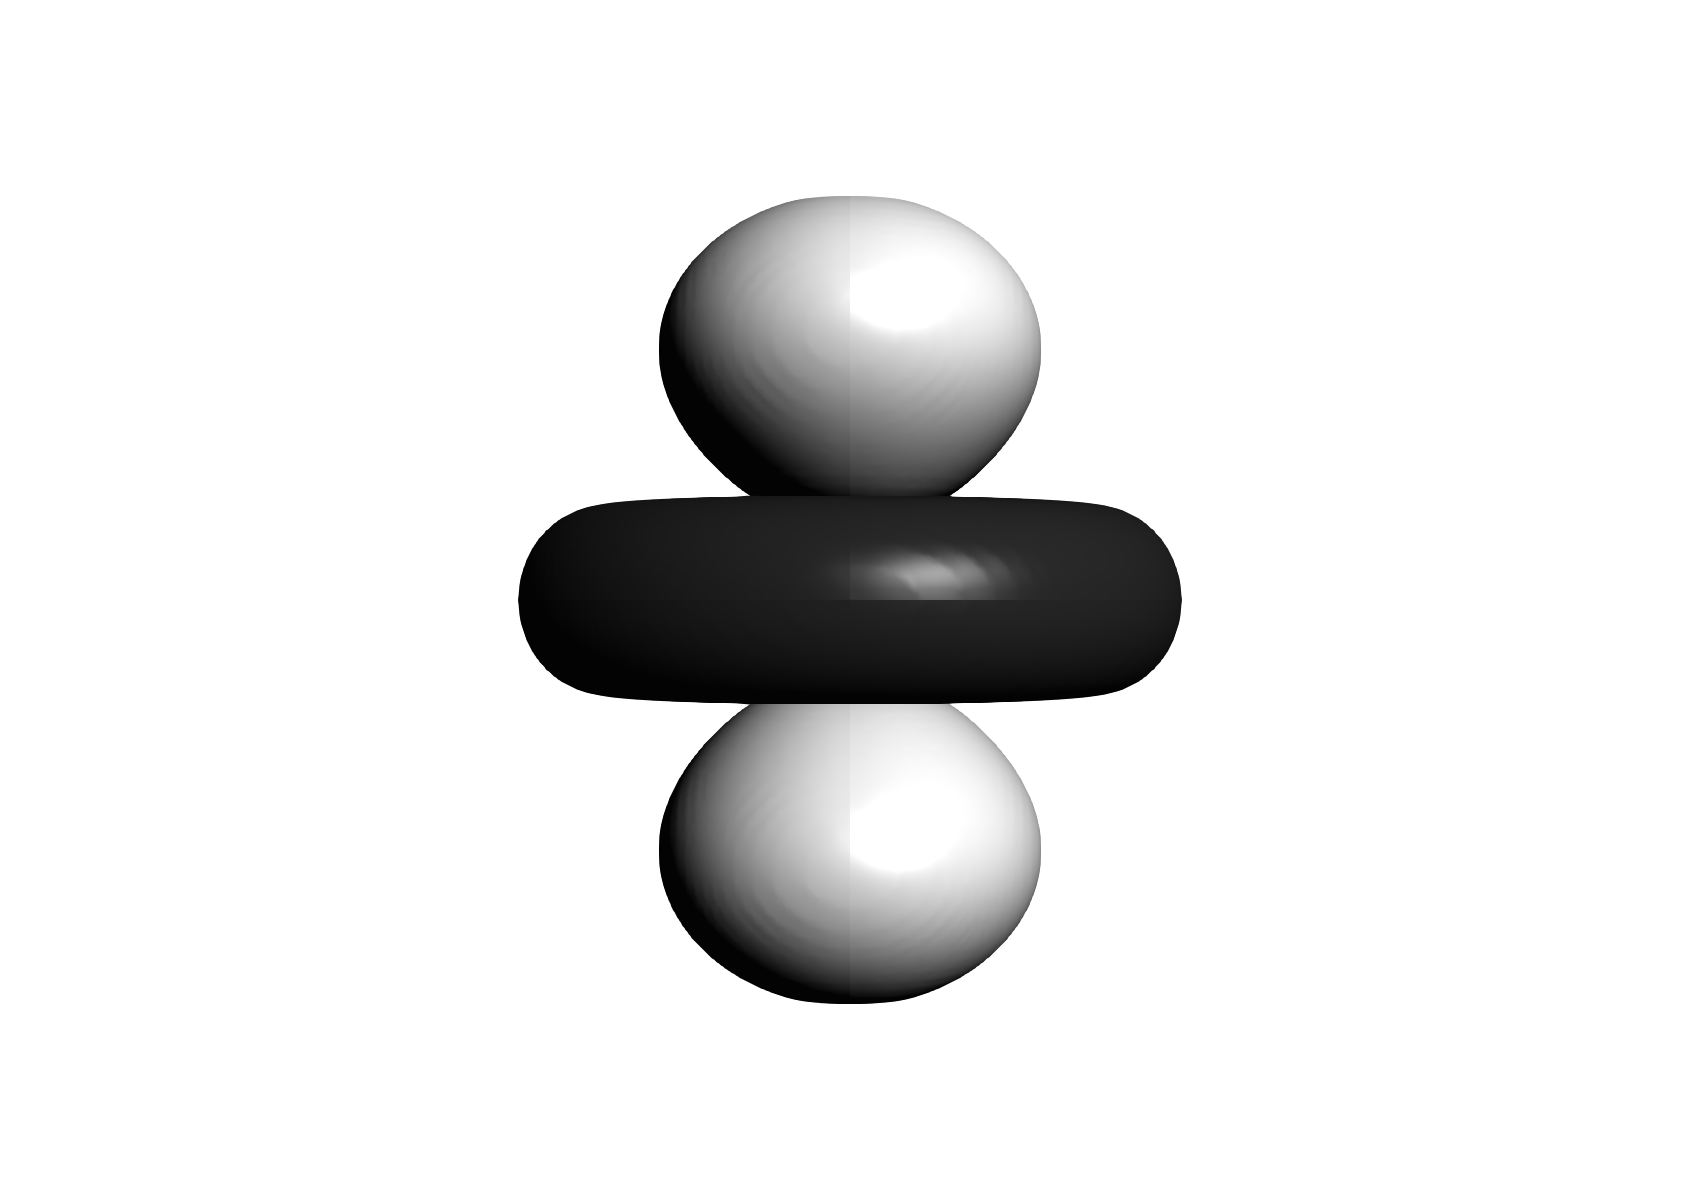
\includegraphics[width=8cm]{dz2.png}
 \caption{Darstellung eines d$_{z^{2}}$-Orbitals \cite{ADF2017authors}.}
 \label{fig:dz2}
\end{dsafigure}

\begin{dsafigure}
 \centering
 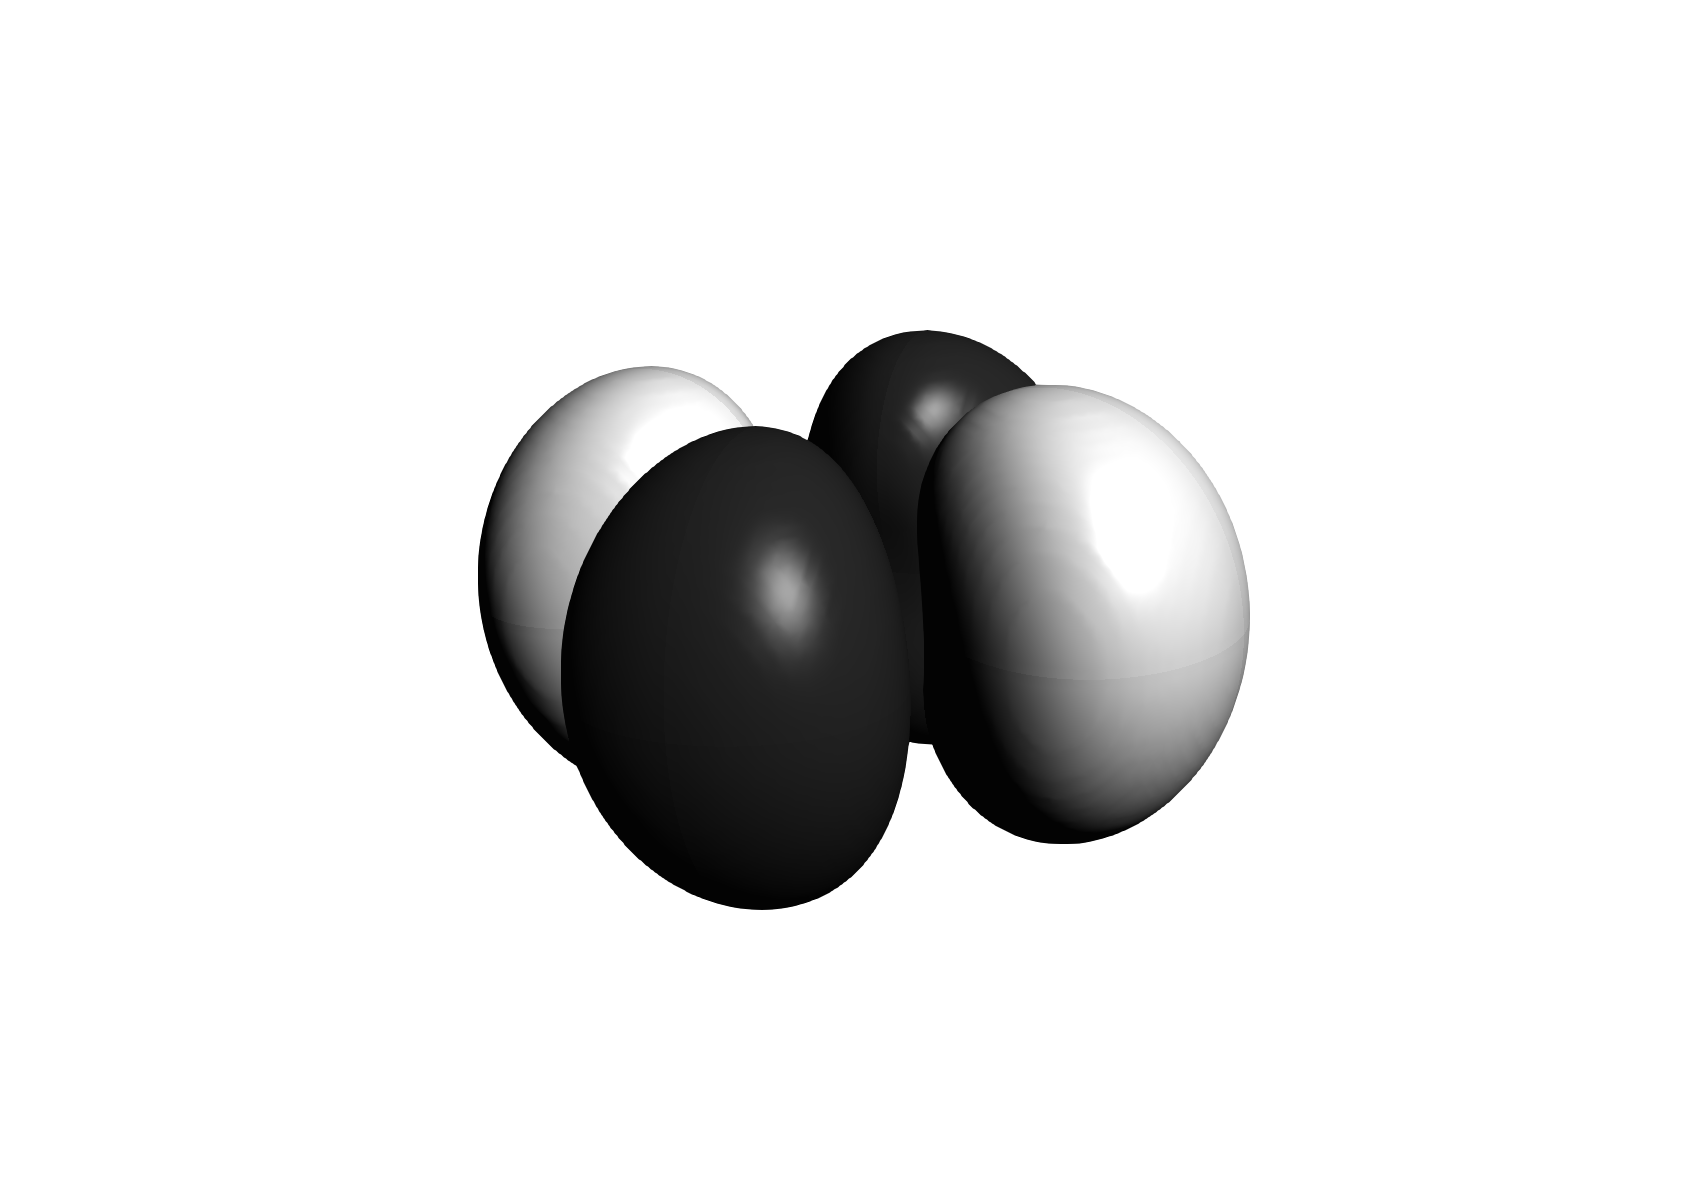
\includegraphics[width=8cm]{dx2-y2.png}
 \caption{Darstellung eines d$_{x^{2}-y^{2}}$-Orbitals \cite{ADF2017authors}.}
 \label{fig:dx2-y2}
\end{dsafigure}

\begin{dsafigure}
 \centering
 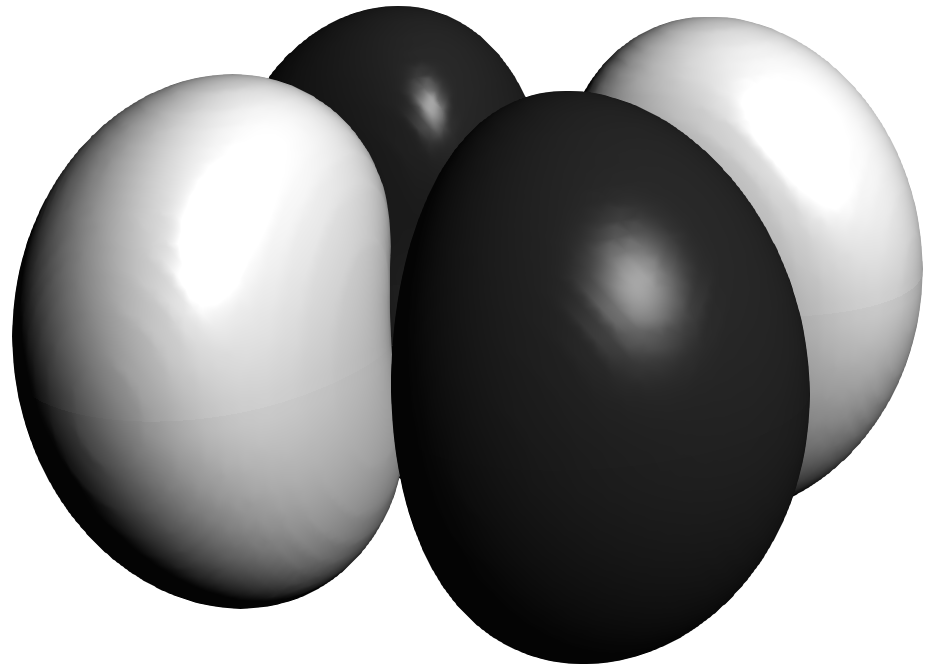
\includegraphics[width=8cm]{dxy.png}
 \caption{Darstellung eines d$_{xy}$-Orbitals \cite{ADF2017authors}.}
 \label{fig:dxy}
\end{dsafigure}

\begin{dsafigure}
 \centering
 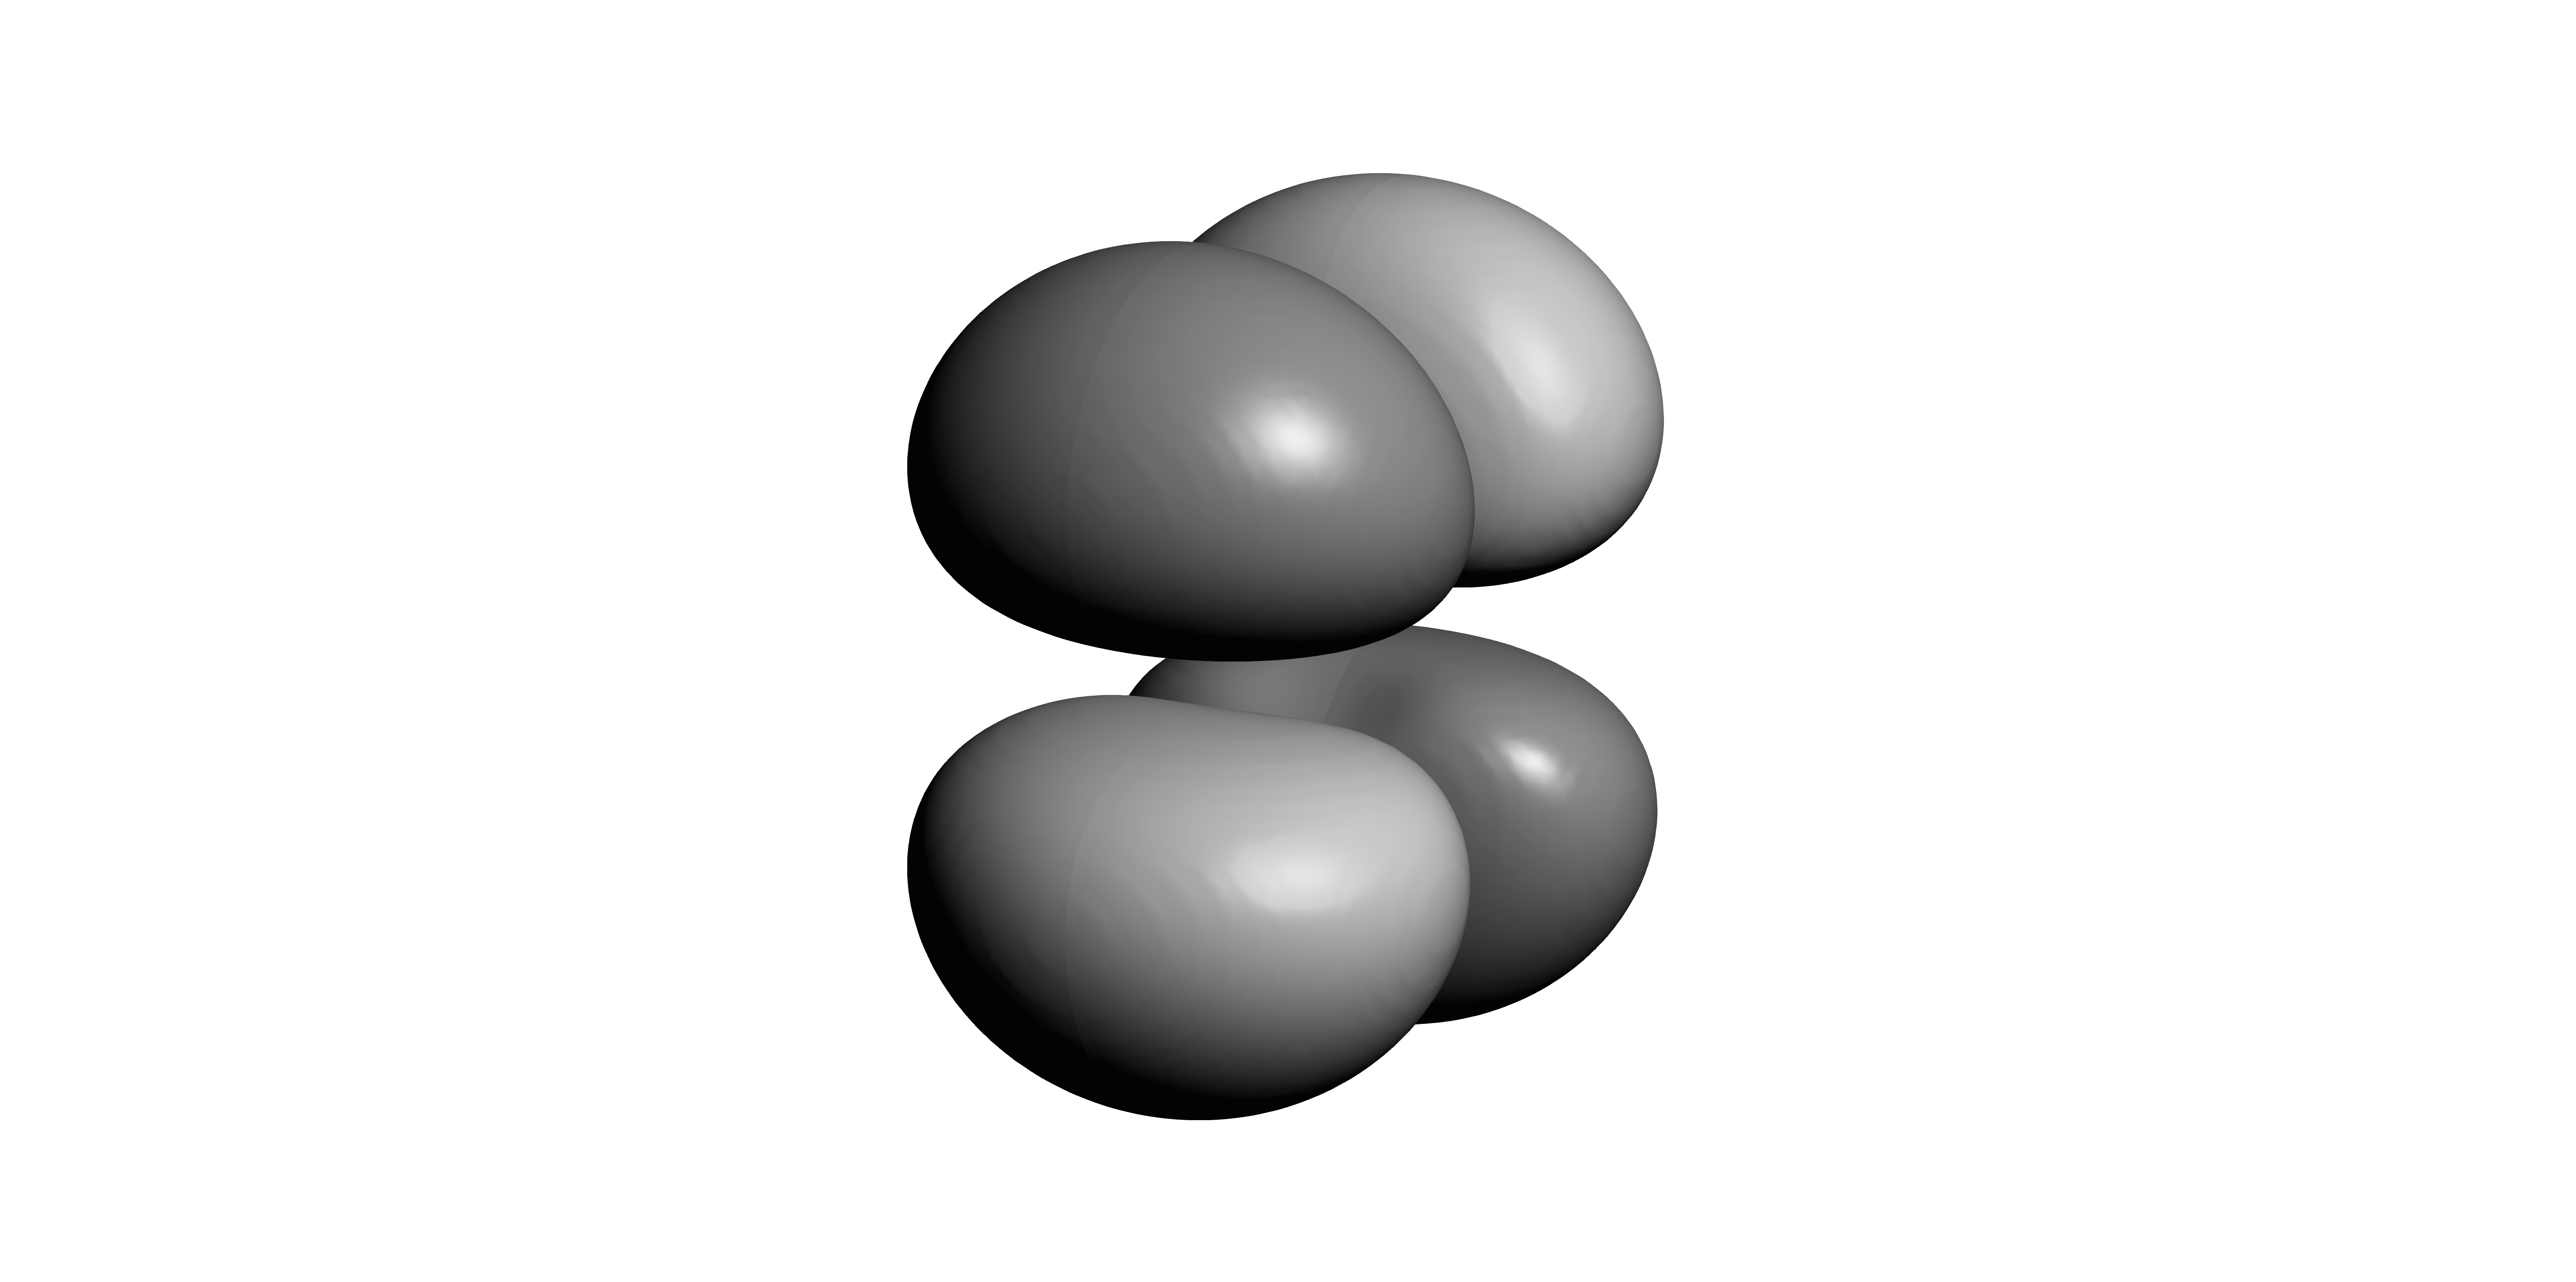
\includegraphics[width=8cm]{dxz.png}
 \caption{Darstellung eines d$_{xz}$-Orbitals \cite{ADF2017authors}.}
 \label{fig:dxz}
\end{dsafigure}

\begin{dsafigure}
 \centering
 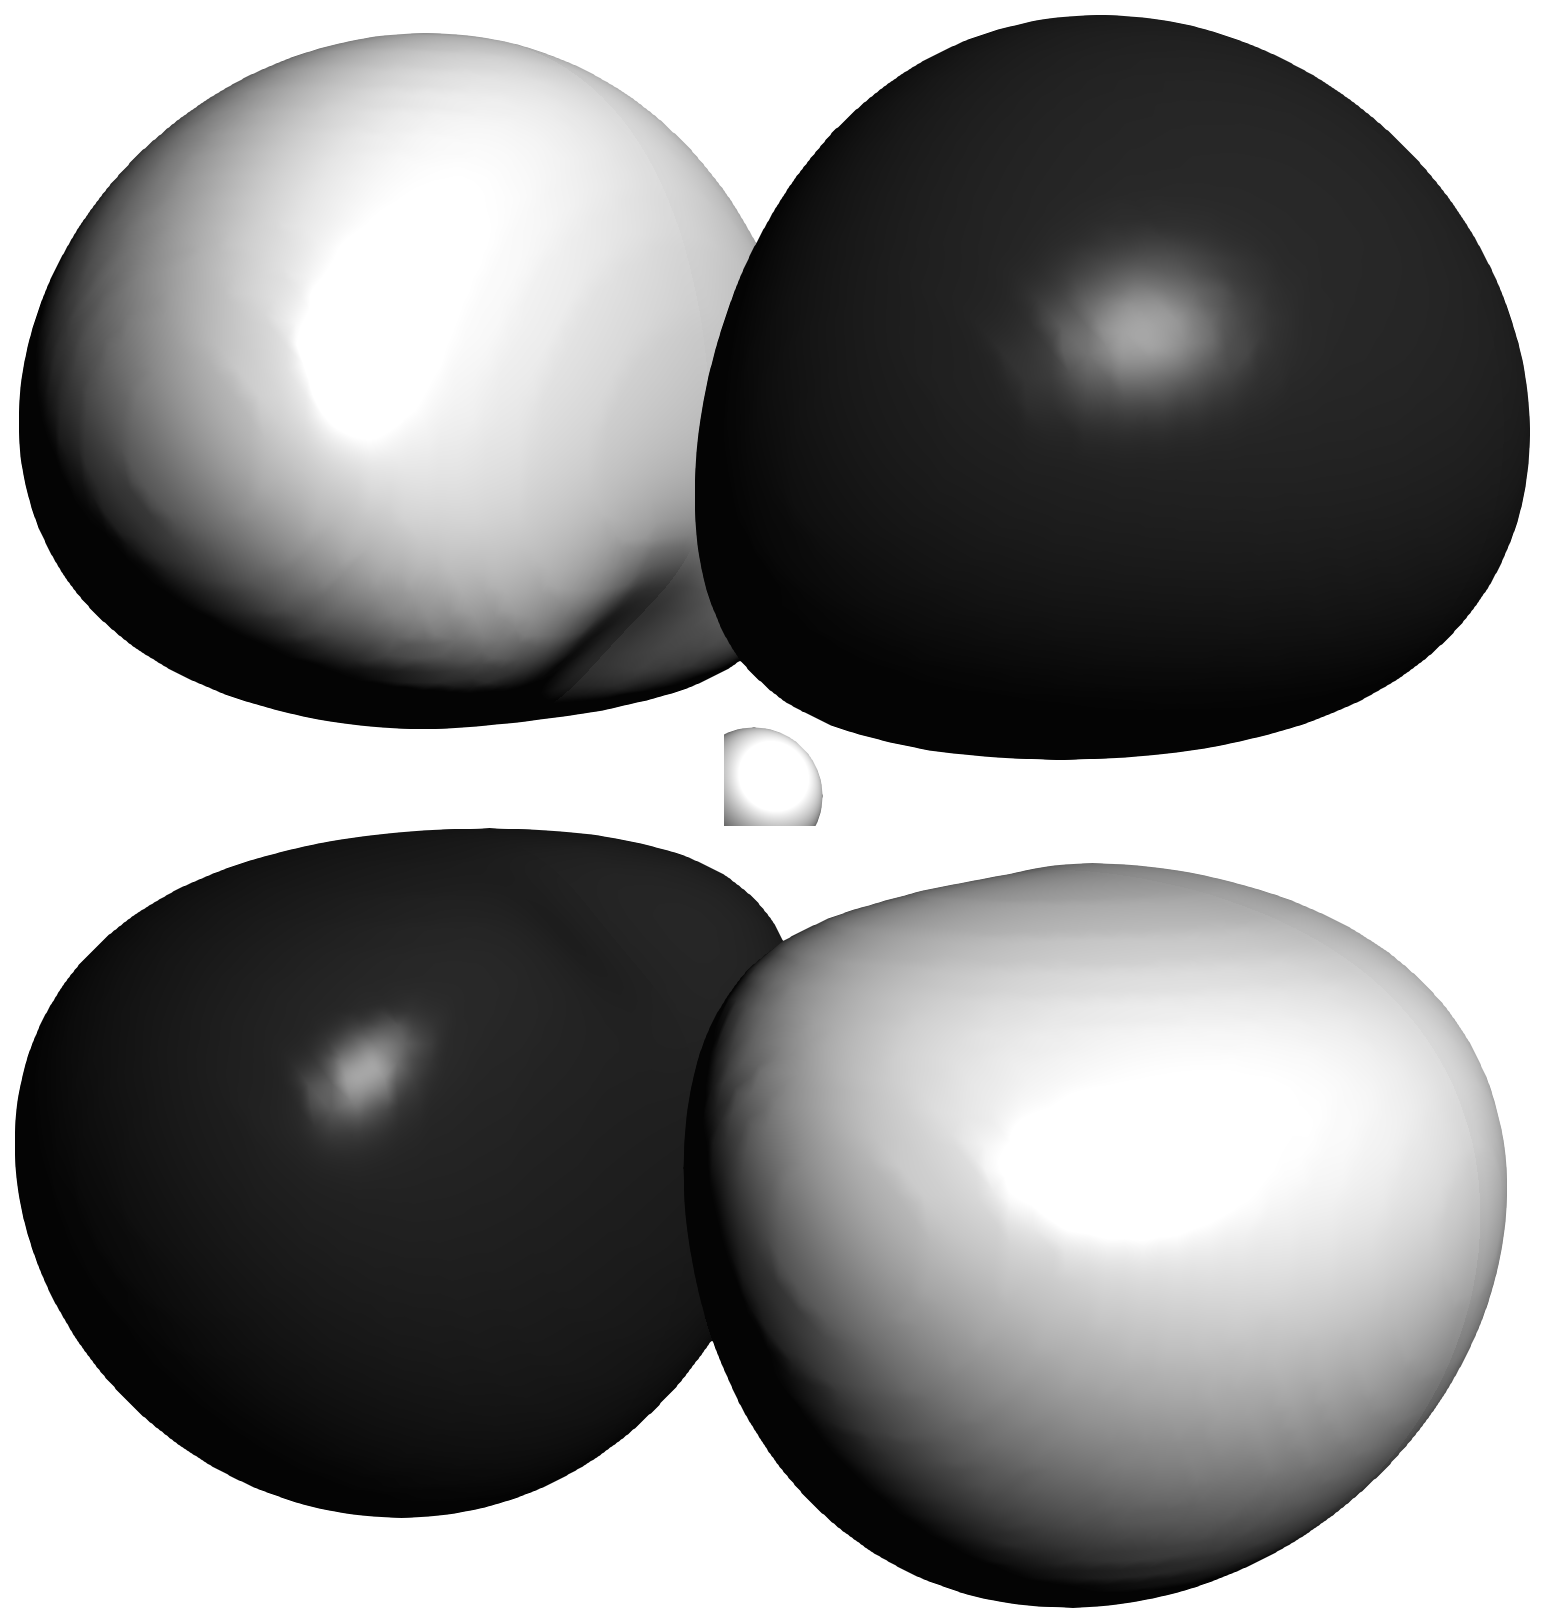
\includegraphics[width=8cm]{dyz.png}
 \caption{Darstellung eines d$_{yz}$-Orbitals \cite{ADF2017authors}.}
 \label{fig:dyz}
\end{dsafigure}


\section{Welle-Teilchen-Dualismus}

Autoren: Patricia Mühren, Kristina Heuser

Das Doppelspaltexperiment mit Photonen und Elektronen sowie der photoelektrische Effekt zeigen auf, dass Licht und Elektronen sowohl Wellen- als auch Teilchencharakter haben.

Zunächst kann das Doppelspaltexperiment mit Kugeln veranschaulicht und theoretisch betrachtet werden. Dabei werden Kugeln von einer Quelle ausgesendet und passieren zwei schmale, parallele Spalten. Auf einem Beobachtungsschirm in einiger Entfernung kann man daraufhin erkennen, dass die Verteilung beziehungsweise die Ankunftswahrscheinlichkeit für klassische Teilchen der Summe der beiden Einzelspaltverteilungen entspricht (vergleiche Abbildung \ref{dsafigure:beispiel1}). Im nächsten Schritt wird das Gedanken-Doppelspaltexperiment mit Wellen ausgeführt. Hier weist die Verteilung ein Interferenzmuster auf. Dies lässt sich dadurch erklären, dass die Maxima der Verteilungsfunktion genau an den Orten konstruktiver Überlagerung liegen (vergleiche Abbildung \ref{dsafigure:beispiel2}). 

\begin{dsafigure}
\centering
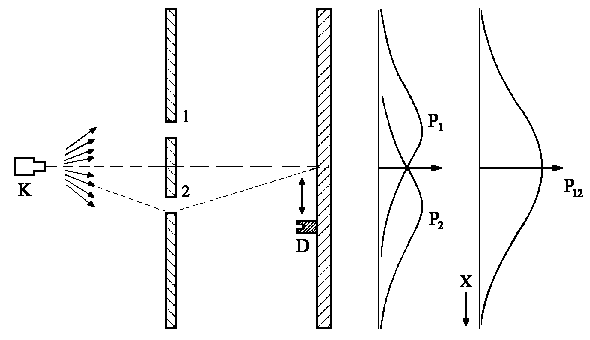
\includegraphics[scale=0.5]{Kugeln.png}
\caption{Das Doppelspaltexperiment mit Kugeln. \cite{Doppelspalt}}
\label{dsafigure:beispiel1}
\end{dsafigure}

\begin{dsafigure}
\centering
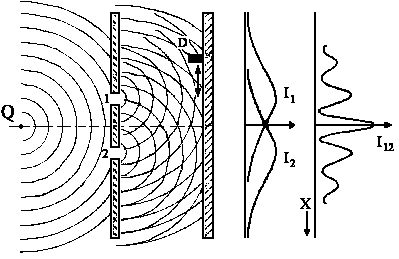
\includegraphics[scale=0.5]{Wellen.png}
\caption{Das Doppelspaltexperiment mit Wellen. \cite{Doppelspalt}}
\label{dsafigure:beispiel2}
\end{dsafigure}

Die Durchführung des Experimentes mit Elektronen zeigt, dass die Verteilungsfunktion der Elektronen nicht der Summe der beiden Einzelspaltverteilungen entspricht, wie sich Abbildung \ref{dsafigure:beispiel3} entnehmen lässt. Daher weisen Elektronen Welleneigenschaften auf. Ebenso zeigt Licht im Doppelspaltexperiment Interferenzen und, einhergehend damit, auch die Eigenschaften einer Welle. 

\begin{dsafigure}
\centering
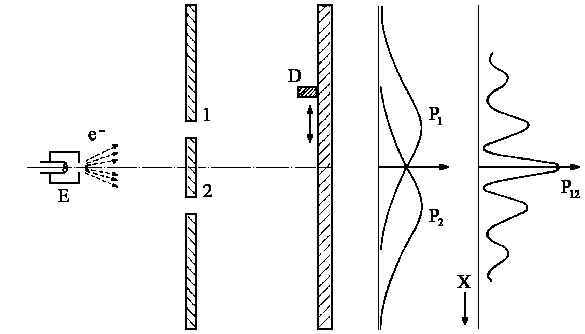
\includegraphics[scale=0.5]{Elektronen.png}
\caption{Das Doppelspaltexperiment mit Elektronen. \cite{Doppelspalt}}
\label{dsafigure:beispiel3}
\end{dsafigure}

Paradoxer Weise illustriert der photoelektrische Effekt, bei dem durch Auftreffen von Licht auf eine Metalloberfläche Elektronen emittiert werden, dass Licht ebenso Teilchencharakter aufweist, der der Wellennatur zuwider zu laufen scheint. Die Beobachtung gleichbleibender Energie der emittierten Elektronen bei zunehmender Intensität des Lichtes widerspricht der aus der klassischen Wellenbeschreibung abgeleiteten Folgerung, dass eine Zunahme der Intensität zu einem Anstieg der kinetischen Energie des herausgelösten Elektrons führen müsste. Dieser Umstand kann mit Teilchencharakter von Elektronen erklärt werden. Analog dazu wird derselbe Versuch mit Elektronen realisiert -- mit dem gleichen Ergebnis wie bei Licht.
Die Tatsache, dass Licht und Elektronen sowohl Wellen-, als auch Teilchencharakter besitzen, wird mit dem Welle-Teilchen-Dualismus addressiert. Sie ist aus einer rein klassischen Anschauung heraus nicht zu erklären und fordert eine neue Theorie \cite{Feynman_lectures70}.



\section{Die Schrödingergleichung}
\authors{Lena Trahe, Lynn Meeder}

Um die Struktur, Energie und Eigenschaften von Atomen und Molekülen zu beschreiben, bedient man sich der Quantenmechanik \cite{Reinhold}.

\subsection{Operatoren und Eigenwertprobleme}

Wendet man einen Operator $\hat{A}$ auf eine Funktion $f(x)$ an, so erhält man eine neue Funktion $g(x)$. Ein bekannter Operator ist zum Beispiel der Differentialoperator  $\frac{d}{dx}$.

Für einen solchen Operator lässt sich eine Eigenwertproblem formulieren, in dem $g(x)= af(x)$ und somit folgende Gleichung gilt:

\begin{equation}
\hat{A}f(x)=af(x)
 \label{OperatorEigenwert}
\end{equation}

Gesucht sind nun die Eigenfunktionen $f(x)$ und die Eigenwerte a, die Gleichung \ref{OperatorEigenwert} genügen.

\subsection{Zeitunabhängige Schrödingergleichung}

Die zeitunabhängige Schrödingergleichung ist das Eigenwertproblem des Hamilton-Operators $\hat{H}$:

\begin{equation}
\hat{H} \psi = E \psi
\end{equation}

Der Hamilton-Operator ist der Operator der Gesamtenergie $E$. Die Gesamtenergie ist die Summe aus kinetischer Energie $T$, die vom Impuls $\vec{p}$ abhängt, und potentieller Energie $V$, die vom Ort $\vec{x}$ abhängt. Analog ist der Hamilton-Operator die Summe aus den Operatoren für die kinetische und die potentielle Energie:

\begin{equation}
\hat{H}(\hat{\vec{p}}, \hat{\vec{x}}) = \hat{T} (\hat{\vec{p}}) + \hat{V} (\hat{\vec{x}})
\label{HamiltonOperatorTV}
\end{equation}

$\hat{\vec{p}}$ ist somit der Impulsoperator und $\hat{\vec{x}}$ der Ortsoperator. Die kinetische Energie $T$ wird in der klassischen Mechanik als $\frac{\vec{p}^2}{2m}$ beschrieben. Den Impulsoperator $\hat{\vec{p}}$ stellt man in der Quantenmechanik nun dar als 

\begin{equation}
\hat{\vec{p}} = -i\hbar \left( 
\begin{array}{c}
\frac{\partial}{\partial x} \\ \frac{\partial}{\partial y} \\ \frac{\partial}{\partial z}
\end{array} \right)
\end{equation}

Durch Einsetzen in den Ausdruck $\hat{T}=\frac{\hat{\vec{p}}^2}{2m}$ erhält man:

\begin{equation}
\hat{T}=-\frac{\hbar^2}{2m}  \left( \frac{\partial ^2}{\partial  x^2}+\frac{\partial ^2}{\partial  y^2}+\frac{\partial ^2}{\partial  z^2}\right)
\end{equation}

Die potentielle Energie hängt nur vom Ort $\vec{x}$ ab und ist deshalb in der Ortsdarstellung ein multiplikativer Operator: $\hat{V}(\hat{x})=\hat{V}(x)$. Die potentielle Energie eines Elektrons mit der Ladung $-e$ im Feld eines Protons mit der Ladung $+e$ beträgt $\hat{V}(x) = -\frac{1}{4 \pi \epsilon_0}\frac{e^2}{r}$. r bezeichnet die Entfernung des Elektrons zum Kern. Für das Wasserstoffatom lautet Gleichung \ref{HamiltonOperatorTV} also:

\begin{equation}
\left[ - \frac{\hbar^2}{2m}  \hat{\vec{\nabla}}^2 -\frac{1}{4 \pi \epsilon_0}\frac{e^2}{r} \right] \psi = E\psi
\end{equation}

Wobei der Operator $\hat{\vec{\nabla}}^2$ gegeben ist als:

\begin{equation}
\hat{\vec{\nabla}}^2 = \frac{\partial ^2}{\partial  x^2}+\frac{\partial ^2}{\partial  y^2}+\frac{\partial ^2}{\partial  z^2}
\end{equation}

Die diskreten Energieeigenwerte $E$ sind hier:

\begin{equation}
E_n=-\frac{m_e e^4}{2\hbar^2}\frac{1}{n^2} \:mit \: n\in \mathbb{N}
\end{equation}

\section{Vielteilchensysteme}
\authors{Joes Biburger, Sophia Ivaschuk}
Vielteilchensysteme, also Systeme, die aus vielen Elektronen (und Kernen) bestehen, sind komplex, da in diesen Wechselwirkungen zwischen mehr als zwei Teilchen berücksichtigt werden müssen. Daraus ergibt sich der folgende Hamilton-Operator:

\begin{equation}
\label{Aufgespalten}
\hat{H} = \hat{T}_{K} + \hat{T}_{e} + \hat{V}_{eK} + \hat{V}_{ee} + \hat{V}_{KK}
\end{equation}
$\hat{T}_{K}$ ist der Operator der kinetischen Energie der Kerne;
$\hat{T}_{e}$ ist der Operator der kinetischen Energie der Elektronen;
$\hat{V}_{eK}$ ist der Operator der Wechselwirkungen zwischen den Elektronen und den Kernen;
$\hat{V}_{KK}$ ist der Operator der Wechselwirkungen zwischen den Kernen
und $\hat{V}_{ee}$ ist der Operator der Wechselwirkungen zwischen den Elektronen.

Um die einzelnen Wechselwirkungen beschreiben zu können, ersetzen wir die Operatoren in Gleichung \ref{Aufgespalten} durch die Terme:

\begin{align}
\begin{split}
\hat{H} =& -\sum^{N}_{i} \frac{\hbar^2}{2m_e} \Delta_{i} + \sum^{N}_{\alpha<\beta}\frac{1}{4\pi \epsilon_0}\,\frac{Z_\alpha Z_\beta e^2}{|\hat{\vec{R}}_\alpha-\hat{\vec{R}}_\beta|}\\
& - \sum^{n}_{i}\sum^{N}_{\alpha}\frac{1}{4\pi \epsilon_0}\,\frac{Z_\alpha e^2}{|\hat{\vec{x}}_i-\hat{\vec{R}}_\alpha|}\\
& + \sum^{n}_{i<j} \frac{1}{4\pi\epsilon_0}\,\frac{e^2}{|\hat{\vec{x}}_i-\hat{\vec{x}}_j|}
\end{split}
\end{align}

In dieser Gleichung steht $Z_{Kern}$ für die Kernladungszahl des betrachteten Kerns; $\Delta_i$ ist der Laplace-Operator; $i$ und $j$ stehen für die jeweils betrachteten Elektronen; $\alpha\,$und$\,\beta$ stehen für die jeweils betrachteten Kerne; $\vec{R}_{Kern}$ und $\vec{x}_{Elektron}$ sind die Raumkoordinaten der betreffenden Teilchen und $e$ ist der Betrag der Ladung eines Protons und eines Elektrons.

Wenn wir die Gesamtenergie des Systems als Summe der kinetischen und potentiellen Energie aller Elektronen mit Ausnahme der Beiträge darstellen, die sich auf andere Elektronen oder nur auf Kerne beziehen, definieren wir eine Näherung, die das System ohne die genannten Wechselwirkungen beschreibt und mit der sich ein erster Ansatz für die Wellenfunktion finden lässt:

\begin{align}
\label{Näherung}
\hat{H}=\sum^{N}_{i=1}\hat{h}(i)
\end{align}

$\hat{h}(i)$ ist hier der Operator für die Energie eines einzelnen Elektrons mit Index $i$. Er vernachlässigt jedoch die Elektron-Elektron-Wechselwirkungen, sowie die kinetische Energie und die Repulsion der Kerne.

Als Lösung der Schrödingergleichung in dieser Näherung des Hamilton-Operators erhalten wir das Hartree-Produkt:
\begin{align}
\psi = \prod^{N}_{i=1} \chi_i
\end{align}
Das Hartree-Produkt wird aus den Spin-Orbitalen $\chi_i, \chi_j,\dots,\chi_N$ konstruiert, für die der Ortsanteil der Einteilchen-Wellenfunktion mit den Spinfunktionen $\alpha(\omega)\,$und$\,\beta(\omega)$ multipliziert wird.


%Die Vielteilchenwellenfunktion $\psi$ wurde nun als Hartree-Produkt, das heißt als das Produkt der Spin-Orbitale $\chi_i$ dargestellt. 
%Zusätzlich zu dieser Näherung muss die Wellenfunktion $\psi$ so aufgestellt werden, dass sie bei der Vertauschung von zwei Elektronen antisymmetrisch ist, um die Ununterscheidbarkeit von Elektronen zu berücksichtigen.

Die Elektronen sind bei diesem Ansatz unterscheidbar und die Wellenfunktion ist unter Vertauschung zweier Elektronen nicht antisymmetrisch. Betrachten wir beispielsweise zwei Elektronen $e_1$ und $e_2$, wobei sich $e_1$ in $\chi_i$ und $e_2$ in $\chi_j$ befindet. Dann lautet das Hartree-Produkt:
\begin{align}
\psi(x_1,x_2)=\chi_i(x_1)\chi_j(x_2)
\end{align} 
Wenn man jetzt die Elektronen vertauscht, erhält man folgenden Ausdruck:
\begin{align}
\psi(x_1,x_2)=\chi_i(x_2)\chi_j(x_1)
\end{align}
Hier sind die Elektronen noch unterscheidbar und $\psi(x_1,x_2)$ ist nicht antisymmetrisch. Deswegen bilden wir eine Linearkombination aus beiden Hartree-Produkten:

\begin{align}\label{eq:lincomb}
\begin{split}
\psi(x_1,x_2)=&2^{-\frac{1}{2}}[\chi_i(x_1)\chi_j(x_2)\\&-\chi_i(x_2)\chi_j(x_1)]
\end{split}
\end{align}

$2^{-\frac{1}{2}}$ ist der Normierungsfaktor.
Hier sind die Elektronen nicht mehr unterscheidbar und $\psi$ ist durch die Subtraktion antisymmetrisch. Außerdem verschwindet die Wellenfunktion, wenn zwei Elektronen im selben Spin-Orbital sind, sodass auch das Pauli-Prinzip befolgt wird. Allgemein lässt sich der Ansatz in Gleichung (\ref{eq:lincomb}) als Determinante einer Matrix schreiben: \cite{Szabo_Ostlund96}
%(siehe Abb.\ref{dsafigure:beispiel}).\\\\\\

\begin{align}
\label{slatermatrix}
\begin{split}
& \psi(x_1,x_2,\dots,x_N) =\\
& \frac{1}{\sqrt{N!}}\left|\begin{matrix}
\chi_i(x_1) & \chi_j(x_1) & \dots & \chi_N(x_1)\\
\chi_i(x_2) & \chi_j(x_2) & \dots & \chi_N(x_2)\\
\vdots&\vdots&\ddots&\vdots\\
\chi_i(x_N) & \chi_j(x_N) & \dots & \chi_N(x_N)\\
\end{matrix}\right|
\end{split}
\end{align}

In Gleichung (\ref{slatermatrix}) ist der antisymmetrische Ansatz für die Vielteilchenwellenfunktionen als Matrix von Einteilchenwellenfunktionen geschrieben. 
Die Zeilen stehen für einzelne Elektronen und die Spalten für einzelne Spin-Orbitale. Diese Determinante wird als Slaterdeterminante bezeichnet.

%\begin{dsafigure}
% \centering
% \includegraphics[width=\columnwidth]{Slaterdeterminante2.png}
% 
% \label{dsafigure:beispiel}
%\end{dsafigure}

\section{Ultramarinblau}
\authors{Sophia Ivaschuk, Gala Gottschalg}

Ultramarinblau ist ein 5000 Jahre altes, anorganisches Farbpigment. Es ist ein Mineral, welches in den Farben Blau, Violett, Pink und Grün vorkommt. Wegen seiner Seltenheit war es früher teurer als Gold. Heute werden pro Jahr 20000 t synthetisch hergestelltes Ultramarinblau verwendet.
Besonders beliebt und geeignet für vielfältige Anwendungen ist Ultramarin durch seine chemischen beziehungsweise physikalischen Eigenschaften. Je nach Pigment ist es bei Temperaturen bis zu 400$^{\circ}C$ und einem pH-Wert zwischen 6 und 9 stabil. Zusätzlich besitzt das geruchlose Ultramarin eine hohe Lichtechtheit, das heißt, die Farbe verblasst auch bei intensiver Bestrahlung nicht. Durch  seine hohe Oberflächenenergie ist der Farbstoff kohäsiv. Er ist nicht mutagen. Somit geht kein Gefahrenpotential von ihm aus, sodass Ultramarin sogar in Kinderspielzeug und Kosmetika verwendet wird. Außerdem findet man ihn  in Seifen und Waschmitteln. 
Früher wurde Ultramarin vor allem in der Kunst verwendet. Besonders beliebt war es bei Malern wegen seiner Lichtechtheit. So verwendeten auch schon die alten Ägypter die Farbe in Totenmasken, bei der Bemalung von Tierfiguren und in Mosaiken.

Um die chemischen und physikalischen Eigenschaften zu verstehen, muss die chemische Struktur des Ultramarins näher beleuchtet werden.
Es besteht aus einem Sodalithkäfig, in welchem die Polysulfidanionen $S_2^{-}$, $S_3^{-}$ und $S_4^{-}$ eingeschlossen sind [Abb.\ref{fig:Ultramarin}].
Der Sodalithkäfig ist ein dreidimensionales Aluminiumsilikatgitter. Dieses besteht aus $SiO_{4}^{-}$- und $AlO_{4}^{-}$-Tetraedern mit zusätzlichen Natrium- und Chloridionen. Die Verhältnisformel des Kristallgitters ist somit $[Na_{8}Al_{6}Si_{6}O_{24}]^{2+}$.
Verantwortlich für die Farbigkeit sind die eingeschlossenen Polysulfidanionen. Diese absorbieren Licht unterschiedlicher Wellenlängen. Je nach dem, wie viele und welche Polysulfidanionen vorliegen, variiert die Farbe. So kommt es zu den unterschiedlichen Farben der Pigmente. 

\begin{dsafigure}
 \centering
 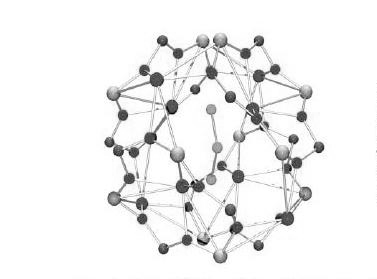
\includegraphics[width=8cm]{Sodalithkaefig.png}
 \caption{Struktur des Ultramarins.}
 \label{fig:Ultramarin}
\end{dsafigure}

Lange Zeit konnte Ultramarin nicht synthetisch hergestellt werden. Die Gewinnung aus den Lagerstätten in Chile und Afghanistan war bei geringer Ausbeute sehr zeitintensiv und aufwändig. Erst 1826 gelang Guimet die Synthese des ersten künstlichen Ultramarins. 1834 wurde die erste Fabrik eröffnet. Zur Herstellung werden Porzellanerde, Feldspat, wasserfreies Natriumcarbonat, Schwefel und ein reduzierendes Mittel verwendet. Zunächst wird die Porzellanerde bei 700$^{\circ}C$ aktiviert. Die Mischung findet danach bei 750$^{\circ}C$ statt. Dabei reagiert das Natriumcarbonat mit Schwefel und dem reduzierenden Mittel zu Natriumpolysulfid, eingelagert in die sodalithische Struktur. Damit ist die Produktion heute relativ kostengünstig und mit einer Ausbeute von 75\% blauem Ultramarin im Rohprodukt recht ertragreich. 
\cite{Buxbaum} 
\cite{Seel}

\section{Sauerstoff und Stickstoff Molekülorbitale}
\authors{David Bürg, Ole Simmering}

Im Folgenden betrachten wir das Sauerstoff- und das Stickstoffmolekül im Lichte der Molekülorbitaltheorie. Bei dieser Betrachtung fällt auf, dass die Elektronenkonfigurationen der Moleküle sich darin unterscheiden, dass die antibindenden-$ \pi $-Orbitale beim Sauerstoffmolekül [Abb. \ref{MO des O2}] einfach und beim Stickstoff [Abb. \ref{MO des N2}] unbesetzt sind. Dadurch ist das Sauerstoffmolekül paramagnetisch, hat Radikalcharakter und befindet sich zudem im Triplettzustand. Bei Stickstoff ist dies nicht der Fall. Dieser Umstand ist darauf zurück zu führen, dass das Sauerstoffatom ein Valenzelektron pro Atom mehr aufweist als das Stickstoffatom. Die gerade genannten Eigenschaften können durch eine Berechnung der Elektronenkonfiguration mit dem quantenchemischen Programm ADF \cite{ADF2017authors} feststellt werden. Die Berechnung wurde mit unrestricted DFT (DZ/B3LYP) für Sauerstoff und restricted DFT (DZ/B3LYP) für Stickstoff durchgeführt. Zuletzt wurde zur Optimierung der Struktur eine Kraftfeldoptimierung der Molekülgeometrie vorgenommen. Die Berechnung liefert die Molekülorbitaldiagramme von Sauerstoff [Abb. \ref{MO_O2_levels}] beziehungsweise Stickstoff [Abb. \ref{MO_N2_levels}].

\begin{dsafigure}
	\centering
	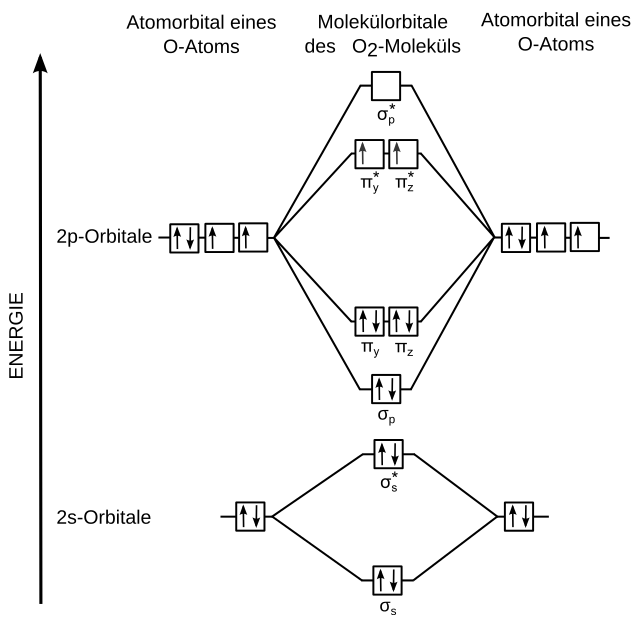
\includegraphics[width=\columnwidth]{MO_O2.png}
	\caption{Molekülorbitaldiagamm eines Sauerstoffmoleküls \cite{MOO2}.}
	\label{MO des O2}
\end{dsafigure}

\begin{dsafigure}
	\centering
	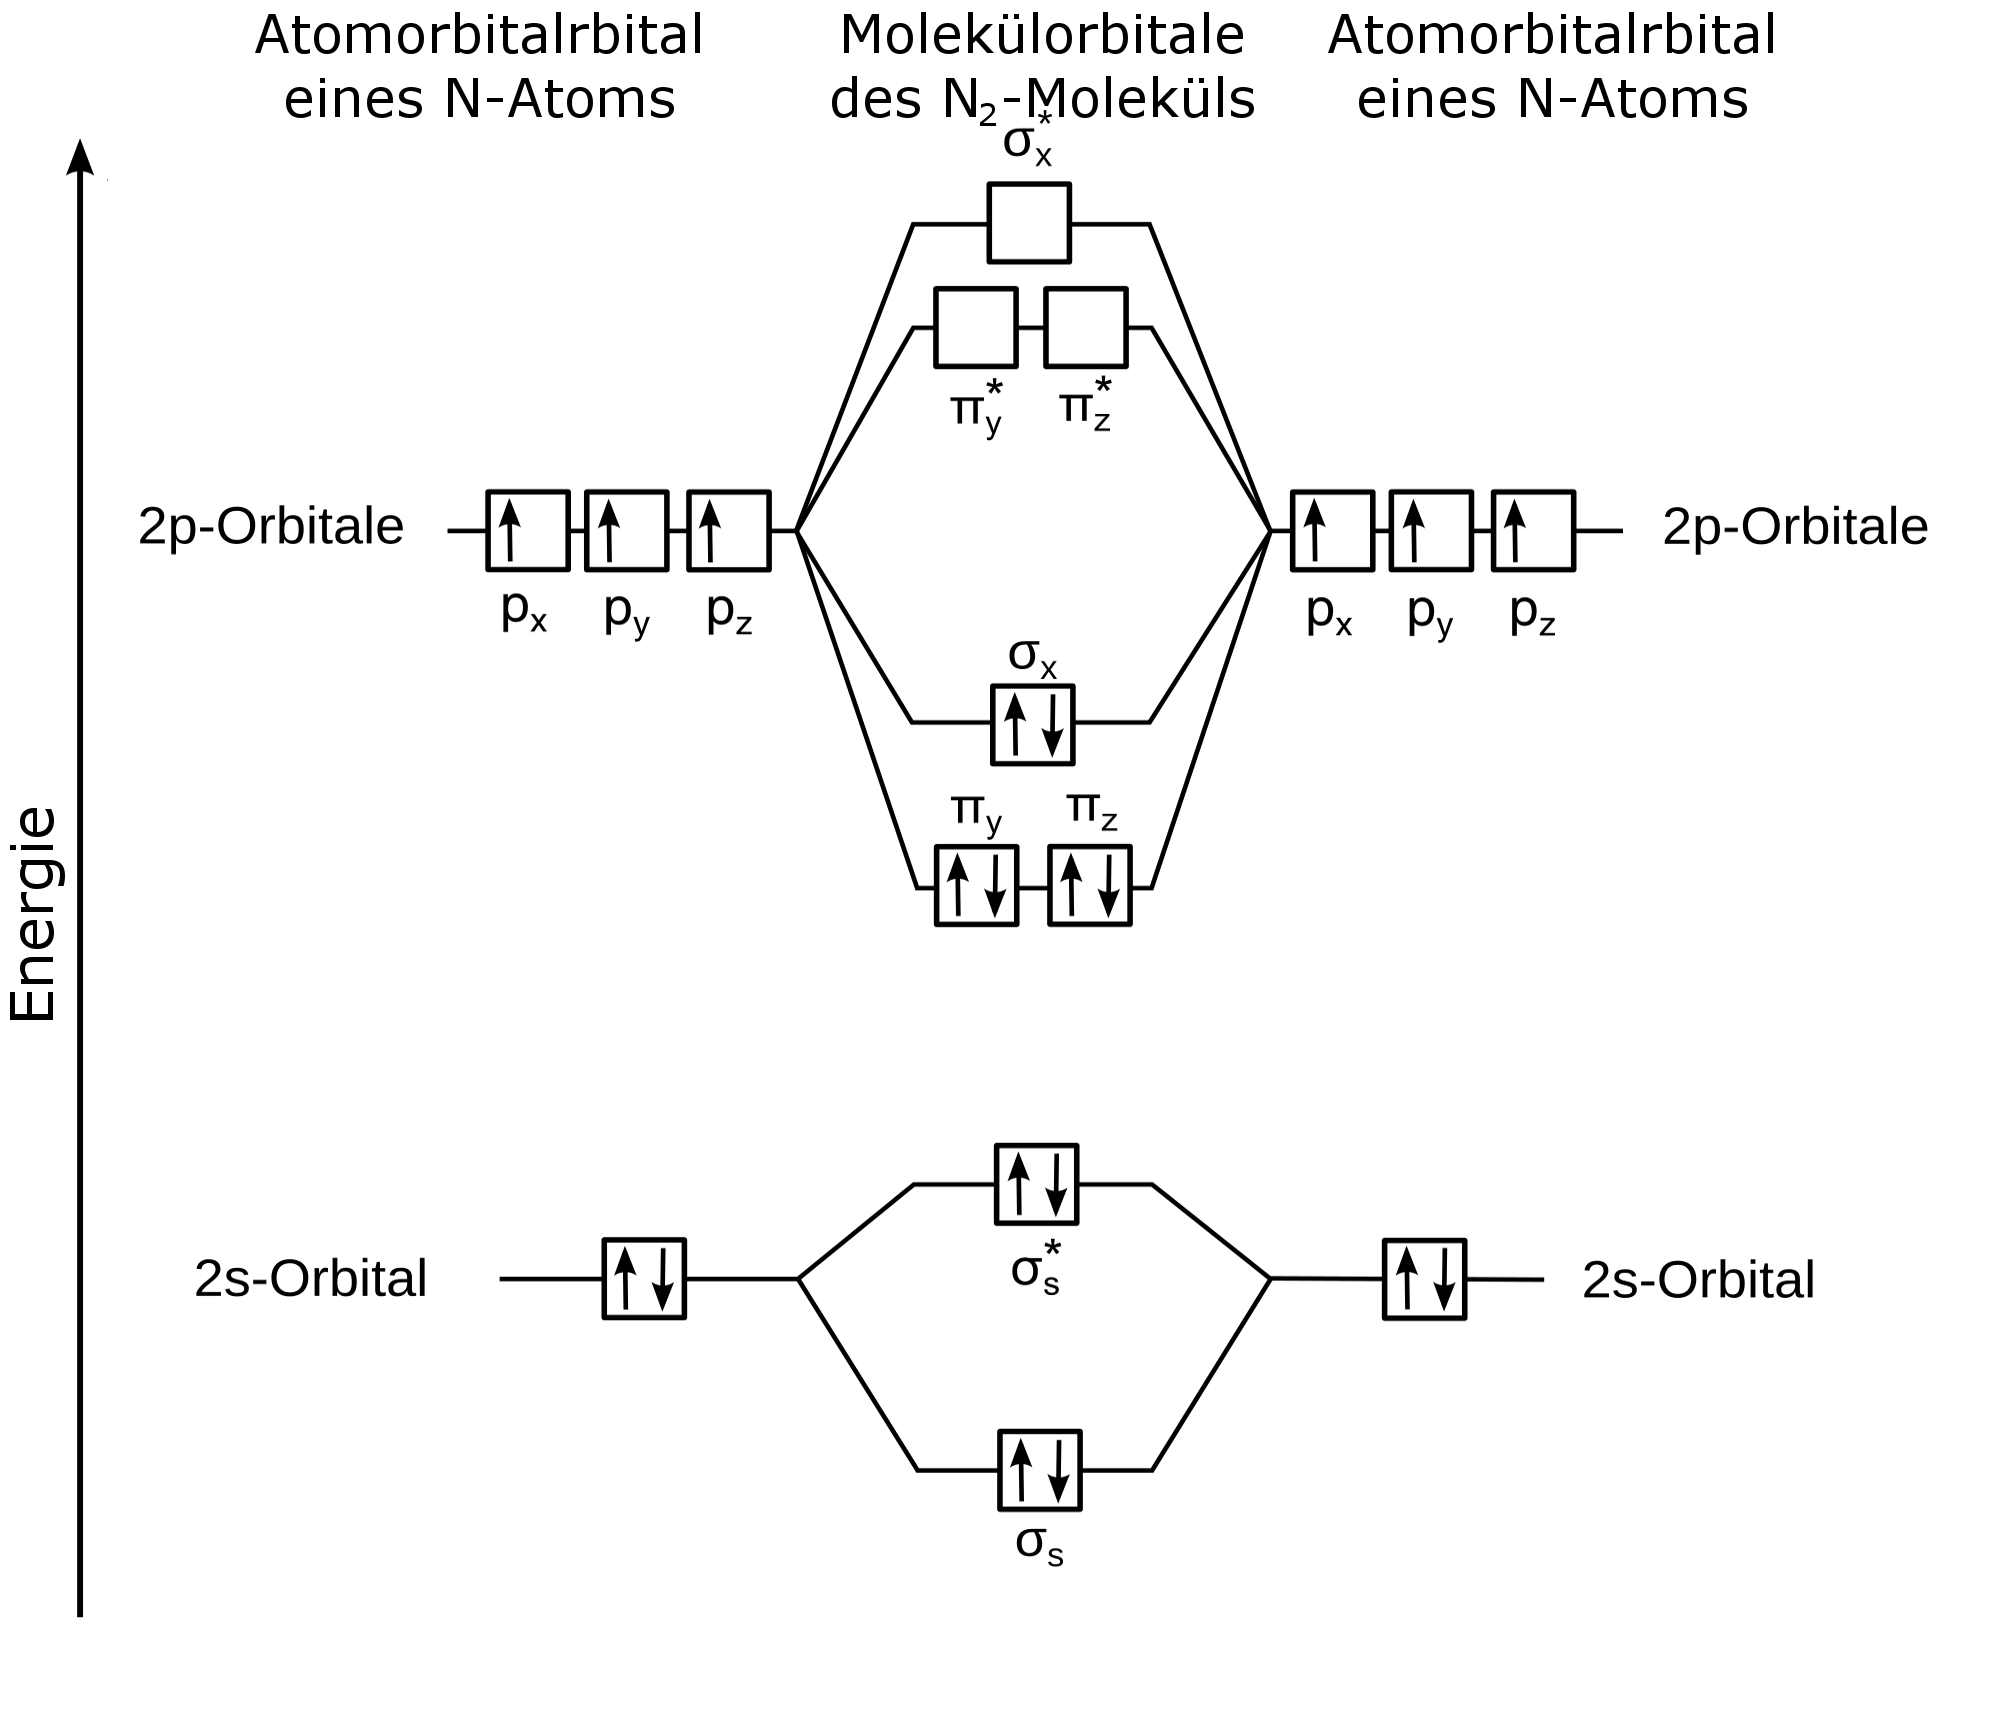
\includegraphics[width=\columnwidth]{MO_stickstoff.png}
	\caption{Molekülorbitaldiagramm eines Stickstoffmoleküls \cite{MON2}.}
	\label{MO des N2}
\end{dsafigure}

\begin{dsafigure}
	\centering
	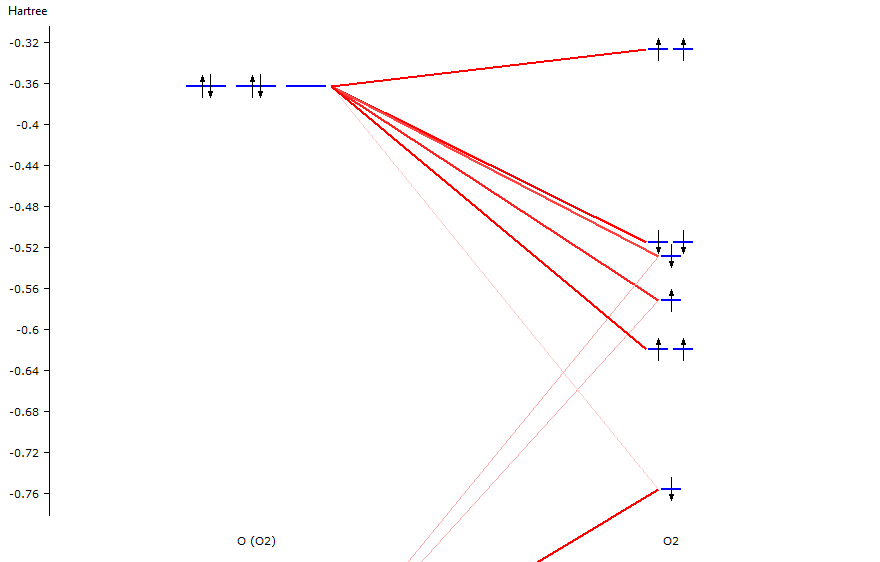
\includegraphics[width=\columnwidth]{MO_O2_levels.png}
	\caption{Mit ADF berechnetes Molekülorbitaldiagramm des Sauerstoffmoleküls.}
	\label{MO_O2_levels}
\end{dsafigure}

\begin{dsafigure}
	\centering
	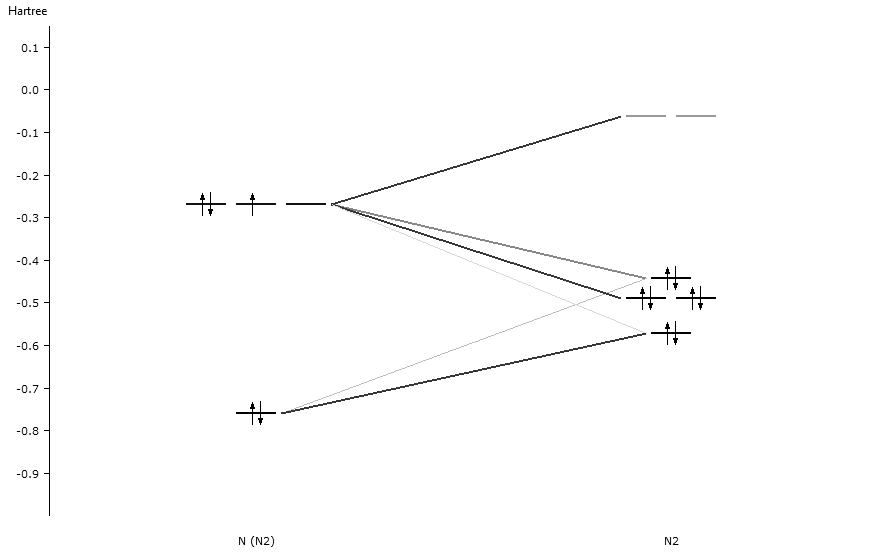
\includegraphics[width=\columnwidth]{MO_N2_levels.png}
	\caption{Mit ADF berechnetes Molekülorbitaldiagramm des Stickstoffmoleküls.}
	\label{MO_N2_levels}
\end{dsafigure}

\section{Molekülorbitale}
\authors{Isabelle Schulte-Herbrüggen, Lena Trahe, Lynn Meeder, Selin Güler}

Die Molekülorbitaltheorie wird genutzt, um die Bindungen innerhalb eines Moleküls quantenmechanisch zu beschreiben. Im Folgenden wird die Theorie auf das Ammoniak- und das Methan-Molekül angewandt.

\subsection{HOMO und LUMO -- freie Elektronenpaare}

Farbigkeit entsteht durch die Absorption von Licht bestimmter Wellenlängen. Diese Wellenlänge wiederum hängt von der Differenz der Energien der verschiedenen Zustände, die man mit den Molekülorbitalen in Näherung beschreiben kann, ab. 
Die Absorption des Lichtes kann man sich als Anregung eines Valenzelektrons in das nächsthöhere Energieniveau vorstellen. Dabei bezeichnet HOMO (Highest Occupied Molecular Orbital) das höchstgelegene besetzte Energieniveau und LUMO (Lowest Unoccupied Molecular Orbital) das nächsthöher gelegene, erste unbesetzte Energieniveau vor der Absorption. Mithilfe des ADF-Programms können sowohl Moleküle gezeichnet als auch Energien berechnet werden. Die Moleküle wurden mit DFT (DZ/B3LYP) berechnet und die Molekülgeometrie wurde mit einem Kraftfeld optimiert.

\begin{dsafigure}
	\centering
	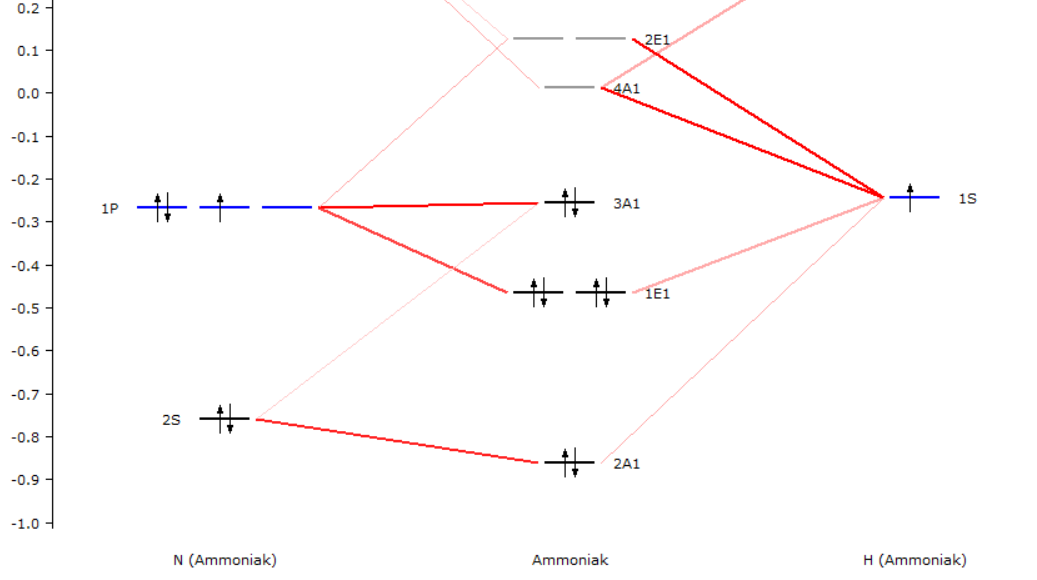
\includegraphics[width=\columnwidth]{AmmoniakLevels.png}
	\caption{Die Energieniveaus der Molekülorbitale von $NH_3$ \cite{ADF2017authors}.}
	\label{levels}
\end{dsafigure}

In Abbildung \ref{levels} sind die verschiedenen Energieniveaus der Molekülorbitale von Ammoniak dargestellt. Links sieht man die Atomorbitale des Stickstoffs, rechts sieht man die Atomorbitale des Wasserstoffs und in der Mitte befinden sich die Molekülorbitale des Ammoniaks. Abbildung \ref{homo} zeigt das höchste besetzte Orbital (HOMO), welches in diesem Fall eine $A_1$-Symmetrie aufweist. Es beschreibt das freie, nicht bindende Elektronenpaar des Ammoniaks. Das erste unbesetzte, energetisch über dem HOMO liegende Orbital ist das beim Ammoniak das ebenfalls $A_1$-Symmetrie aufweisende LUMO, welches in Abbildung \ref{lumo} dargestellt ist.

\begin{dsafigure}
	\centering
	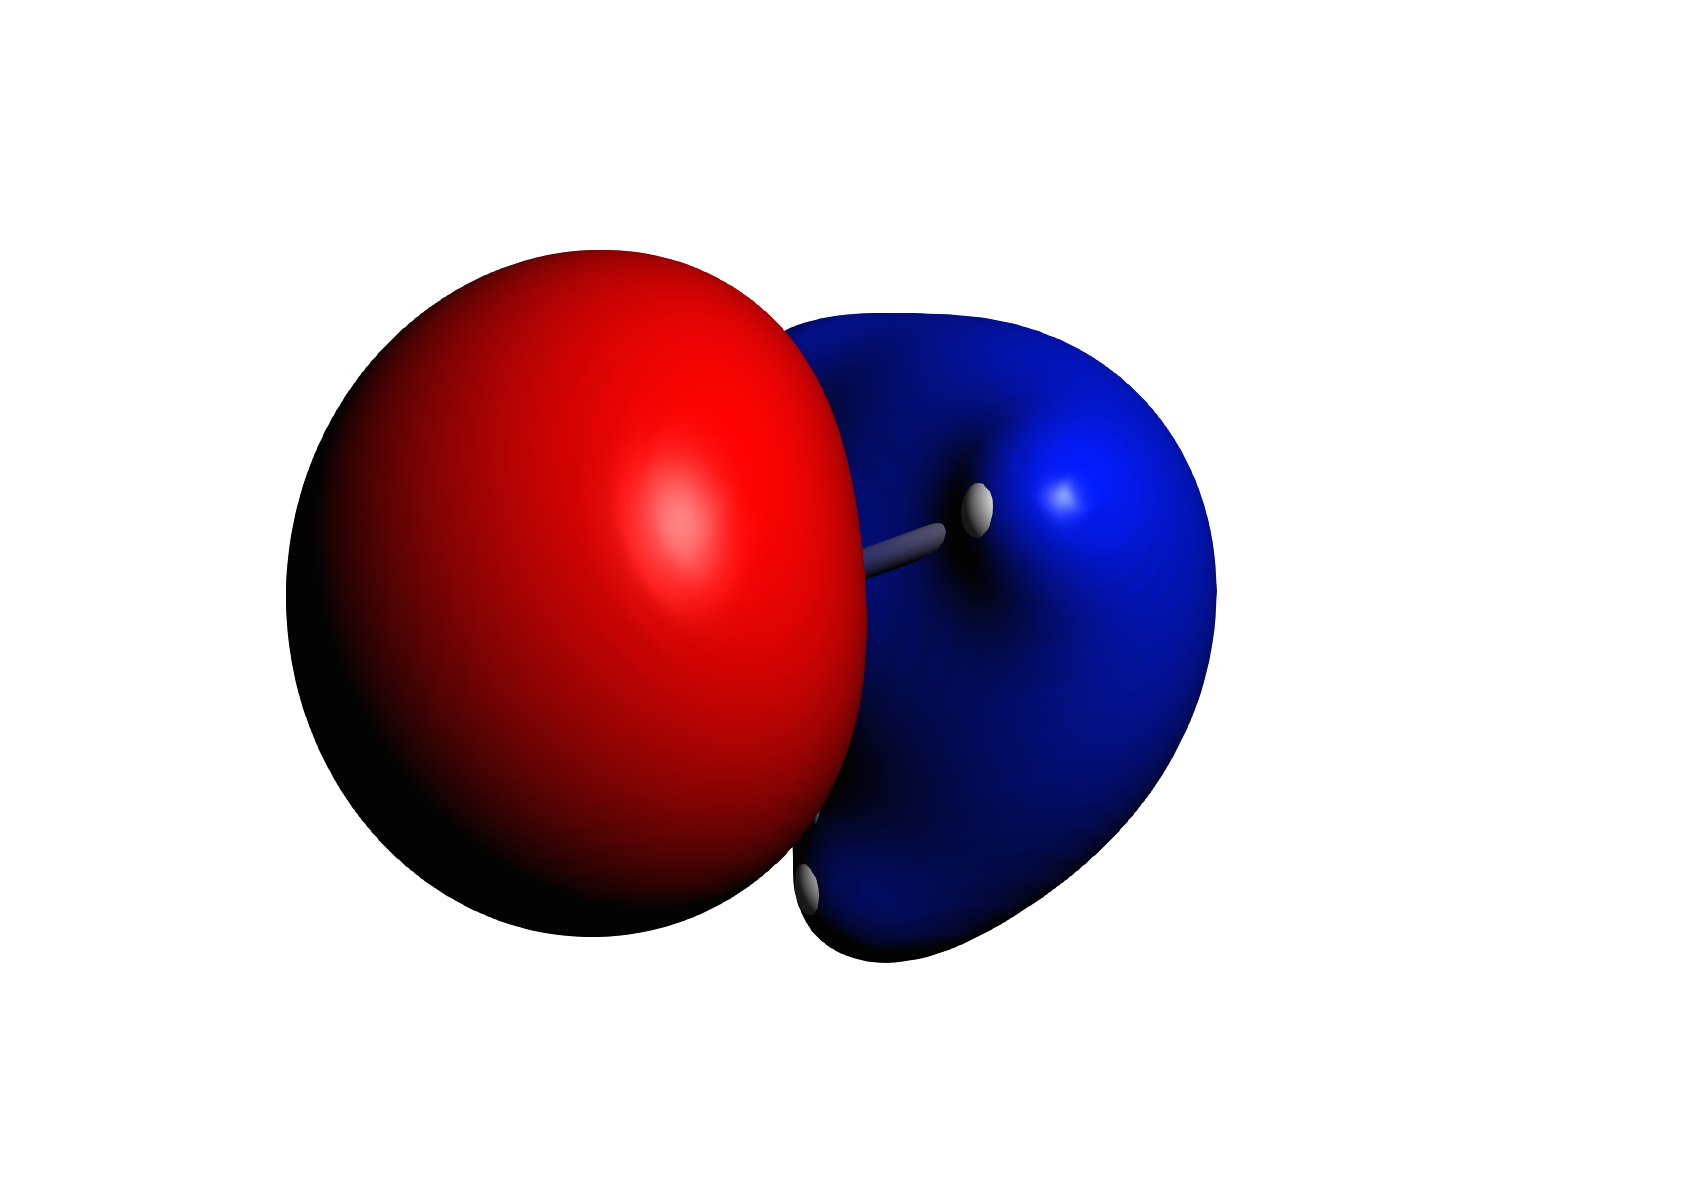
\includegraphics[width=4cm]{Orbital_3A1.png}
	\caption{HOMO des $NH_3$ \cite{ADF2017authors}.}
	\label{homo}
\end{dsafigure}

\begin{dsafigure}
	\centering
	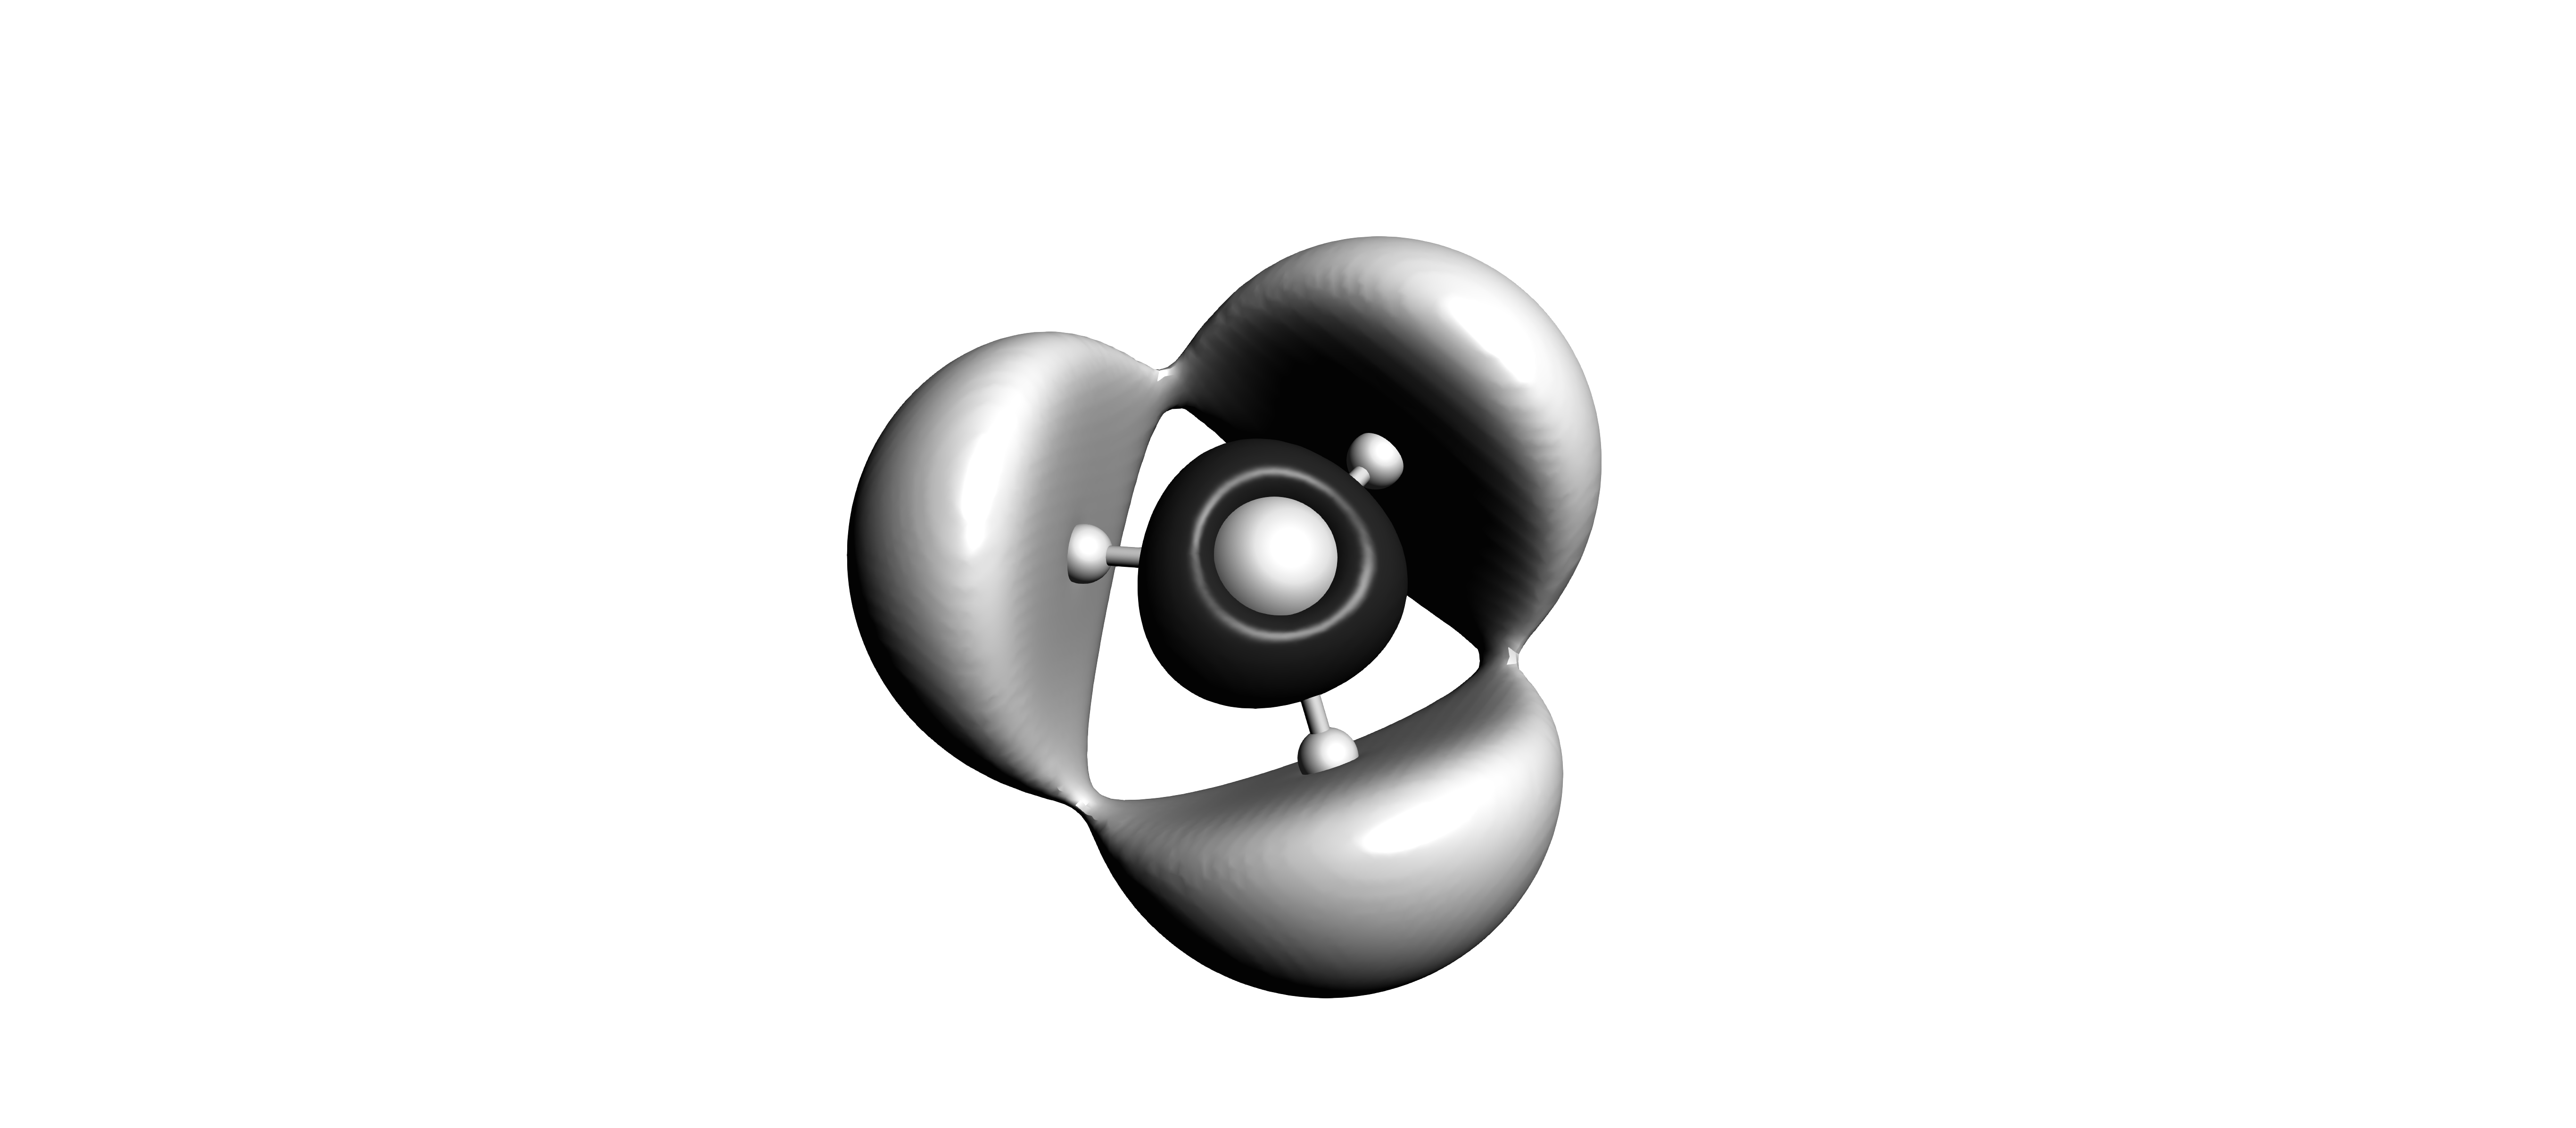
\includegraphics[width=4cm]{Orbital_4A1.png}
	\caption{LUMO des $NH_3$ \cite{ADF2017authors}.}
	\label{lumo}
\end{dsafigure}

\subsection{Hybridisierung versus Molekülorbitaltheorie}

In zahlreichen Experimenten zur Bestimmung von Winkeln und Bindungsabständen wurde belegt, dass ein Methanmolekül die Form eines Tetraeders besitzt. Alle Bindungen sind somit identisch.
Die Berechnung eines Methanmoleküls zeigte einen Unterschied zwischen den Energieniveaus der vier höchsten besetzten Molekülorbitale. Die Abbildung \ref{EnergieniveausMethan} verdeutlicht dies.

\begin{dsafigure}
 \centering
 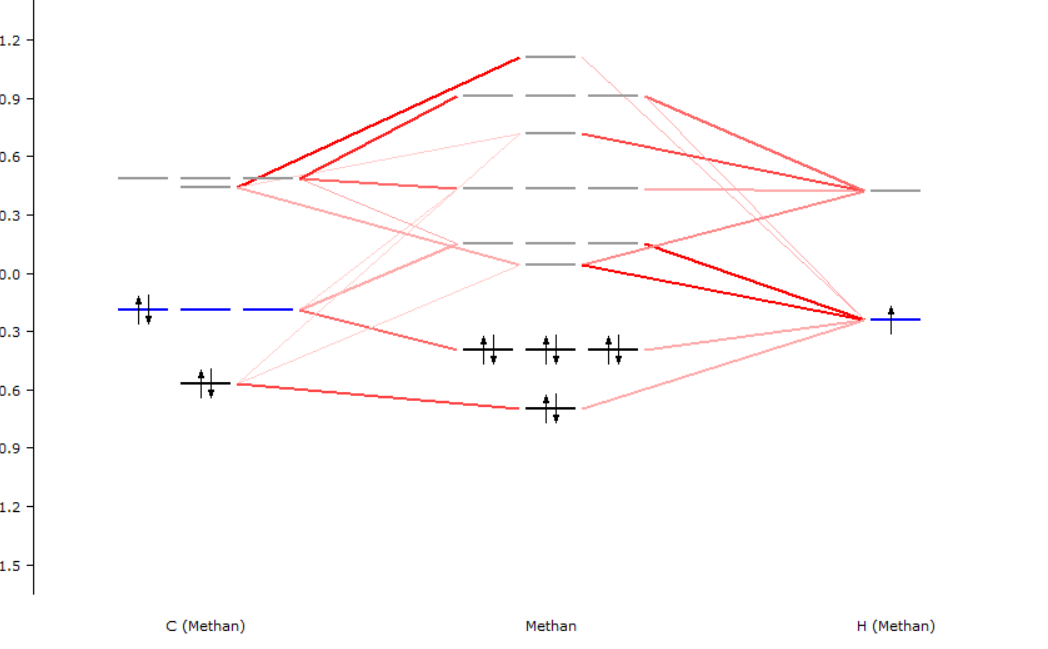
\includegraphics[width=\columnwidth]{LevelsMethan.png}
 \caption{Energieniveaus des Methanmoleküls \cite{ADF2017authors}.}
 \label{EnergieniveausMethan}
\end{dsafigure}

Links sind die Atomorbitale eines Kohlenstoffatoms und rechts die Atomorbitale eines Wasserstoffatoms abgebildet. In der Mitte sind dann die Molekülorbitale des Methanmoleküls dargestellt. Die horizontalen Linien repräsentieren die Energieniveaus der verschiedenen Orbitale. Dabei wird deutlich, dass ein Molekülorbital eine geringere Energie als die übrigen drei der vier höchsten besetzten Molekülorbitale besitzt. 
Es zeigt sich ein Unterschied zwischen dem Modell der Hybridorbitale und der von ADF genutzten Molekülorbitaltheorie, durch die man auch quantitative Informationen wie die Energien erhält. Das Modell der Hybridorbitale hingegen definiert die Energien nicht, sondern liefert qualitative Aussagen zur Geometrie und Bindungsverhältnissen. Hybridorbitale resultieren bloß aus der Anpassung der Atomorbitalbasis an die Tertaederstruktur des Moleküls. Für die Molekülorbitale werden hingegen die Energien einzelner Elektronen optimiert. 
Es handelt sich also um zwei unterschiedliche Betrachtungsweisen.
Insgesamt beschreiben beide Modelle die Struktur des Methanmoleküls als Tetraeder. In Abbildung \ref{OrbitalMethan} ist eins der drei HOMOs dargestellt.

\begin{dsafigure}
 \centering
 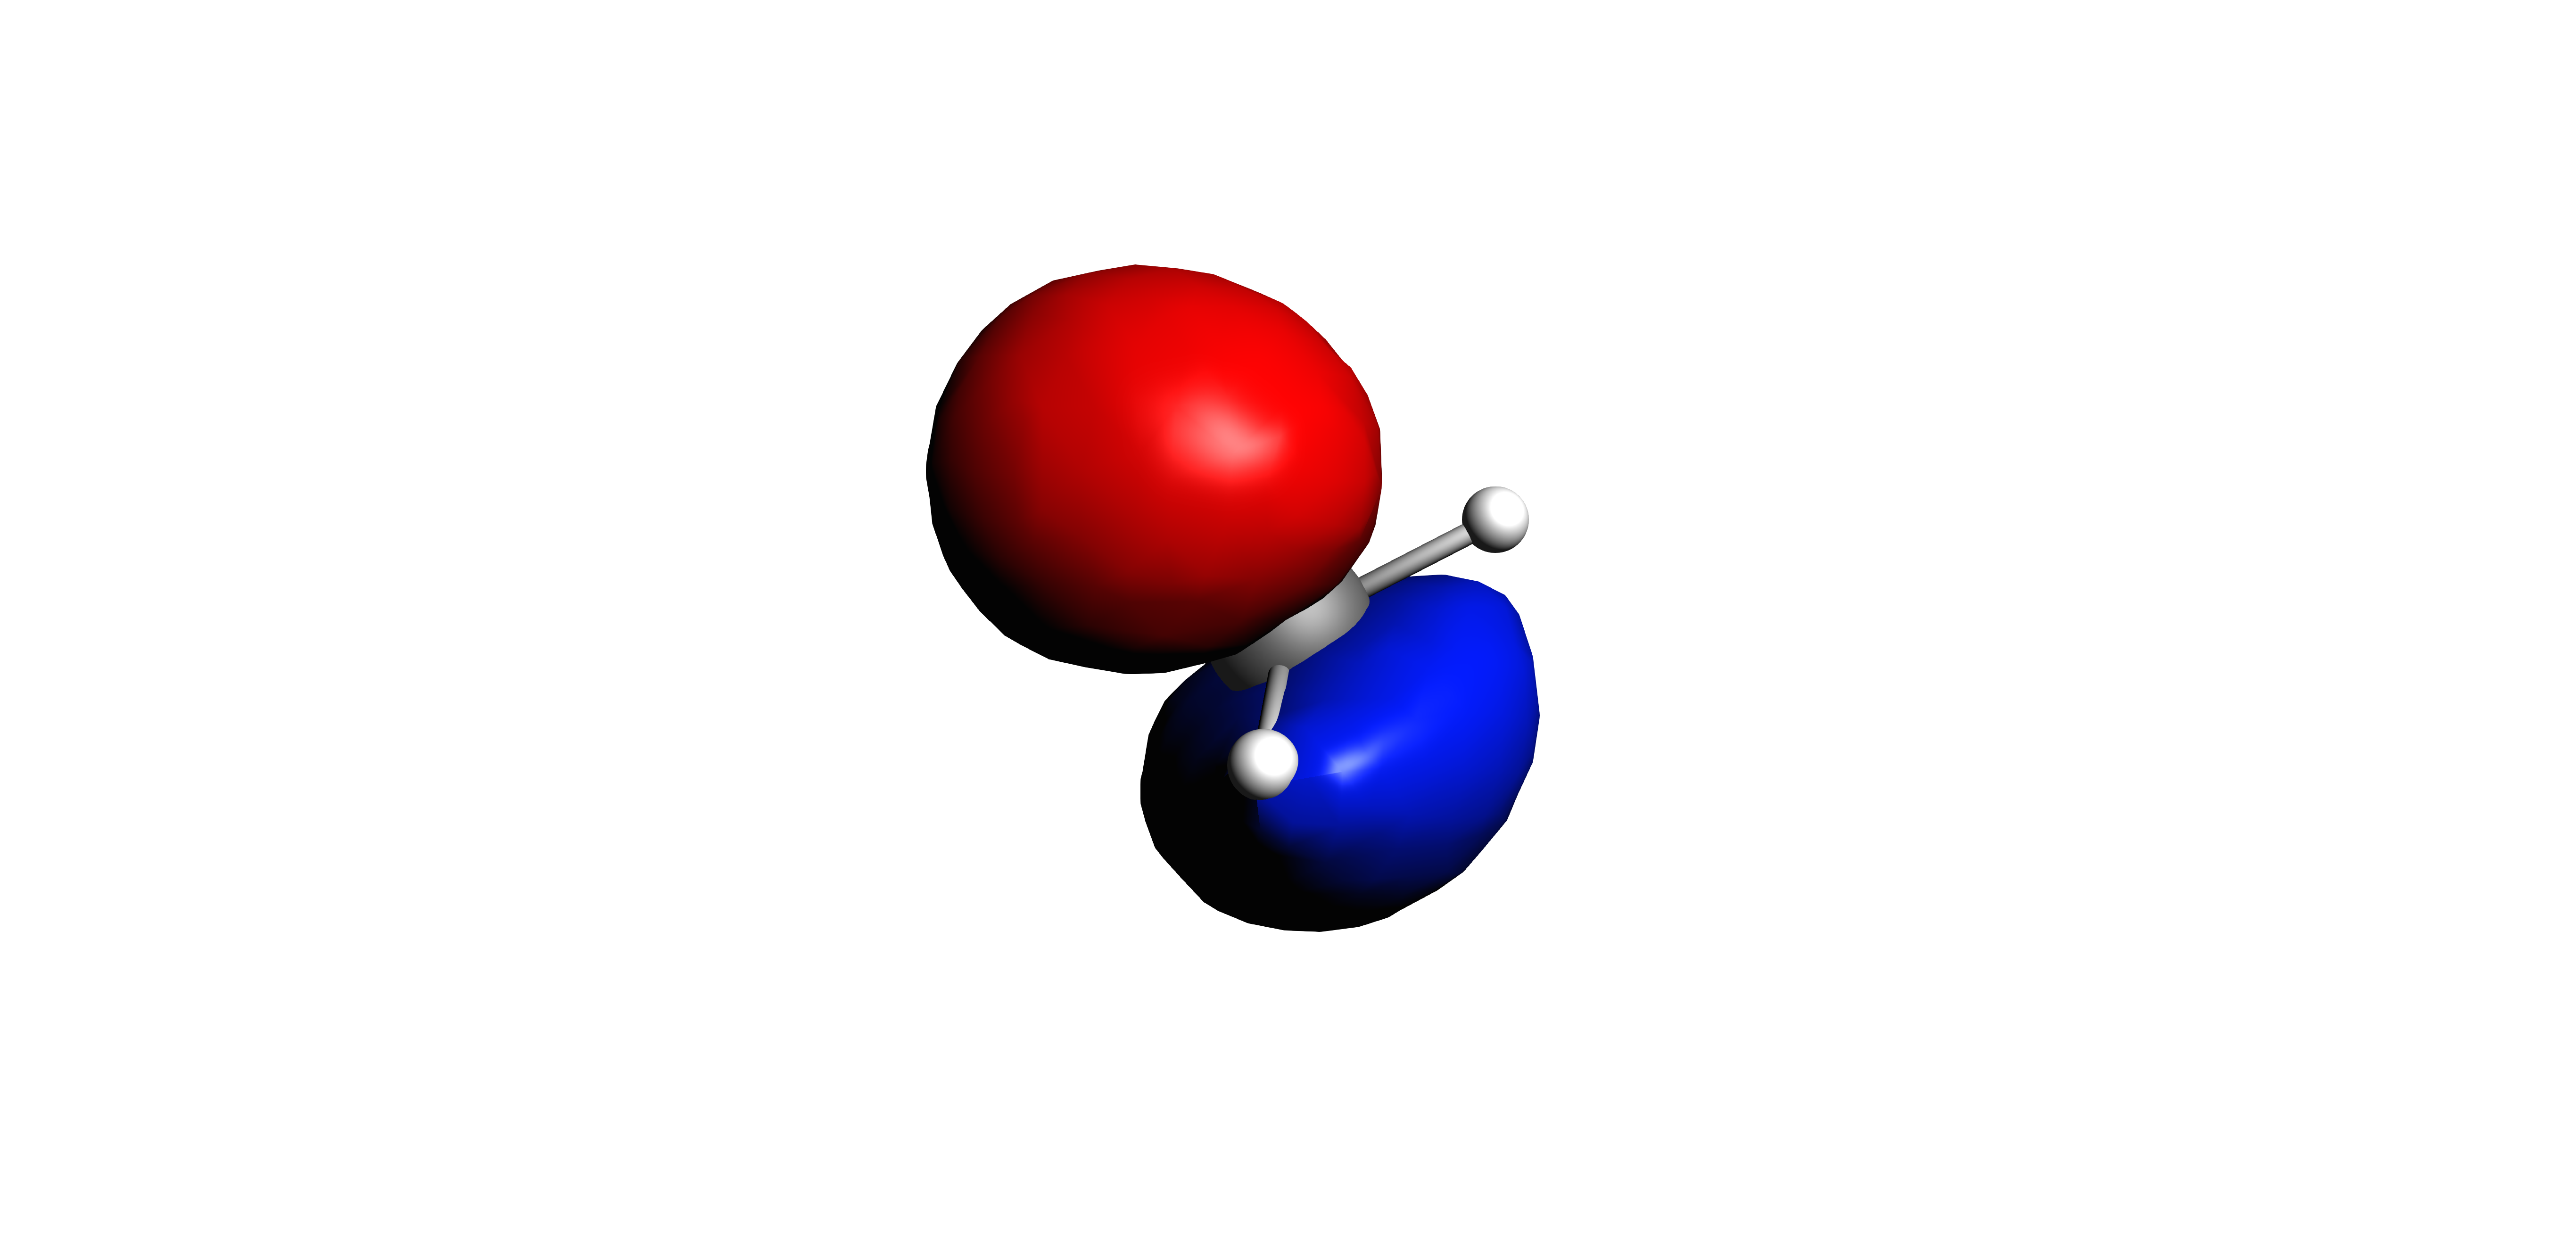
\includegraphics[scale=0.04]{MethanA5.png}
 \caption{Eines der drei HOMOs eines Methanmoleküls \cite{ADF2017authors}.}
 \label{OrbitalMethan}
\end{dsafigure}


\section{Koordinationsverbindungen II - Ligandenfeldtheorie}
\authors{Lynn Meeder, Patricia Mühren}

Die Kristallfeldtheorie beschreibt Koordinationsverbindungen, wobei die Liganden klassisch betrachtet werden und das Zentralatom/-ion quantenmechanisch beschrieben wird. Ein genaueres Modell ist die Ligandenfeldtheorie, in der sowohl das Zentralatom/-ion als auch die Liganden sowie ihre Wechselwirkungen quantenmechanisch betrachtet werden.

\subsection{Ligandenfeldtheorie und 18-Elektronen-Regel}

Analog zur Oktettregel lässt sich die 18-Elektronen-Regel für Nebengruppenelemente formulieren. Wenn das System 18 Valenzelektronen hat, so ist die Komplexbildung stabil \cite{Huheey}.

Die Liganden sorgen auch in diesem Modell, genau wie bei der Kristallfeldtheorie, für eine Aufspaltung der Energieniveaus der $d$-Orbitale des Zentralatoms/-ions. Dabei bilden die $d_{z^2}$- und $d_{x^2-y^2}$-Orbitale des Zentralatoms/-ions mit zwei symmetrieadaptierten Linearkombinationen (SALCs) der Liganden zwei bindende und zwei antibindende Orbitale. Die bindenden Orbitale liegen auf einem energetisch niedrigeren Niveau und werden als $e_g$-Orbitale bezeichnet. Auf einem höheren Energieniveau liegen die antibindenden $e^*_g$-Orbitale. Die energetisch niedriger liegenden $d_{xy}$-, $d_{xz}$- und $d_{yz}$-Orbitale  werden als $t_{2g}$-Orbitale bezeichnet und sind nicht bindend.

Das unbesetzte $s$-Orbital des Zentralatoms/-ions bildet mit einem der SALCs der Liganden das komplett symmetrische $a_{1g}$-Orbital und das entsprechende antibindende $a^*_{1g}$-Orbital. Die drei unbesetzten $p$-Orbitale des Zentralatoms/-ions bilden mit drei SALCs der Liganden die bindenden, dreifach entarteten $t_{1u}$-Orbitale und ebenfalls die entsprechenden antibindenden $t^*_{1u}$-Orbitale.

Die Aufspaltungsenergie $\Delta_0$ beschreibt die Energiedifferenz zwischen den $e^*_g$- und $t_{2g}$-Orbitalen (siehe Abbildung \ref{Level}).

\begin{dsafigure}
	\centering
	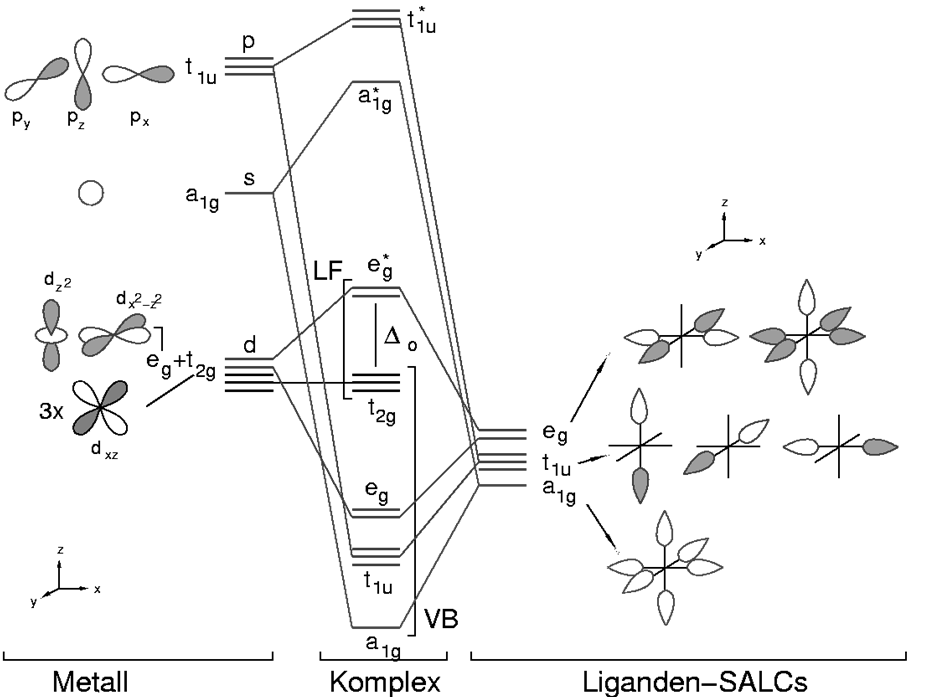
\includegraphics[width=\columnwidth]{EnergielevelKomplex.png}
	\caption{Die Molekülorbitale einer oktaedrischen Koordinationsverbindung \cite{Chemie_der_Metalle}}
	\label{Level}
\end{dsafigure}

Wie in Abbildung \ref{Level} sichtbar, gibt es sechs bindende und drei nicht bindende Orbitale. Die stärkste Bindung erhält man also, wenn diese neun Orbitale voll -- also mit 18 Elektronen -- besetzt sind. Damit lässt sich nun die 18-Elektronen-Regel begründen. 

Diese Regel gilt nun allerdings wie Abbildung \ref{Level}  nur für oktaedrische Komplexverbindungen. Bei anderen Koordinationsgeometrien unterscheidet sich das Molekülorbitalschema und dadurch kann eine andere Zahl an Valenzelektronen stabil sein.



\section{Hückeltheorie}

Autoren: David Bürg, Isabelle Schulte-Herbrüggen

Die Hückeltheorie wurde in den 1930er Jahren von Erick Hückel entwickelt. \cite{Reinhold} Sie erlaubt eine einfache Beschreibung von konjugierten Doppelbindungssystemen. Die Methode arbeitet mit vielen Näherungen. Daher ist sie zwar ungenau, aber einfach anzuwenden. Sie baut auf der Näherung von $\pi$-Molekülorbitalen und deren Energien über Linearkombinationen von p-Atomorbitalen auf. Die Linearkombinationen können mit:

\begin{align}
 \psi_{i} = \sum \limits_{k=1}^n c_{ik} \chi_k 
\end{align}

beschrieben werden. Der Koeffizient $c_{ik}$ gibt hierbei an, wie  stark die einzelnen Atomorbitale $\chi_k$ am Molekülorbital $\psi_i$ beteiligt sind. Die Koeffizienten $c_{ik}$ lassen sich über die Summen:

\begin{align}\label{eq:hueckel}
  \sum \limits_{k=1}^n (H_{jk}-\epsilon_i S_{jk}) c_{ik} = 0
\end{align}

bestimmen. $H_{jk}$ ist das Hamiltonmatrixelement, $S_{jk}$ das Überlappmatrixselement und $\epsilon_i$ ist die Energie des Molekülorbitals. Mit Gleichung (\ref{eq:hueckel}) kann nun die Hückelmatrix formuliert werden. Dabei wird angenommen, dass die Hamiltonmatrixelemente aller Kohlenstoffatome gleich sind, sowie dass die Wechselwirkungen aller nächsten Nachbarn gleich sind. Zusätzlich vereinfacht man die Beschreibung noch weiter, indem die Wechselwirkungen zwischen nicht-nächsten Nachbarn komplett vernachlässigt werden. Aufgrund dieser Vereinfachungen sind die Ergebnisse, die man durch Anwenden der Hückeltheorie erhält, grobe Näherungen.


Indem man fordert, dass die Determinante der Hückelmatrix verschwindet, erhält man einen Satz gekoppelter Gleichungen, deren Lösung die Koeffizienten $c_{ik}$ und die Orbitalenergien $\epsilon_i$ liefert. So kann nun die Energiedifferenz zwischen HOMO und LUMO mit:

\begin{align}
  \Delta E = \epsilon_{LUMO} - \epsilon_{HOMO}
\end{align}

berechnet werden. Diese Energiedifferenz erlaubt eine grobe Abschätzung der ersten Anregungsenergie des Moleküls.

Beschreibt man das 1,3-Butadien-Molekül mit der Hückelthoerie, erhält man die in Abbildung  \ref{fig:Hueckel_Butadiene} dargestellten Molekülorbitale.

\begin{dsafigure}
 \centering
 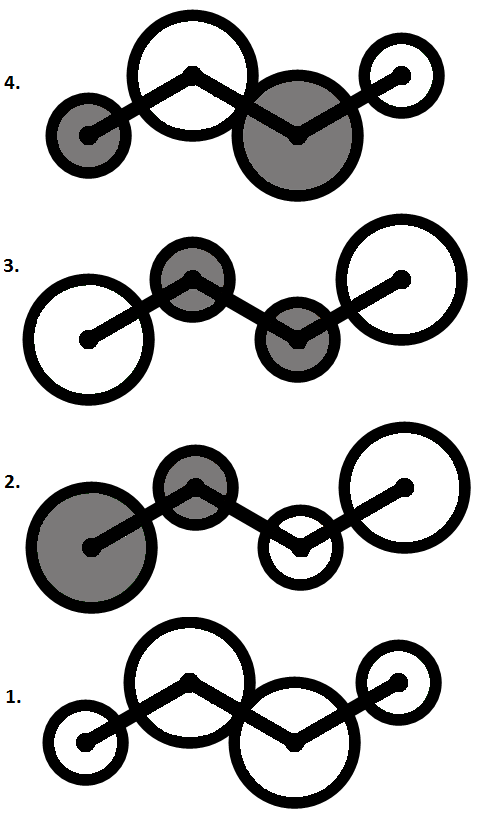
\includegraphics[width=8cm]{Hueckel_Butadiene.png}
 \caption{Aufsicht auf ein 1,3-Butadienmolekül. Schematische Darstellung der Hückelmolekülorbitale von 1,3-Butadien.}
 \label{fig:Hueckel_Butadiene}
\end{dsafigure}

Die Radien der Kreise entsprechen den Koeffizienten $c_{ik}$, während Weiß und Grau die Positivteile beziehungsweise Negativteile beschreiben. Das erste Orbital ist das energetisch günstigste Molekülorbital von Butadien, da es nur bindende Wechselwirkungen aufweist und keine Knotenebene besitzt; es ist ein bindendes Orbital. Das zweite Orbital hingegen weist zwei bindende Wechselwirkungen und eine Knotenebene auf. Es handelt sich auch hier um ein bindendes Orbital. Beim dritten un vierten Orbital handelt es sich um antibindende Orbitale. Das dritte Orbital zeigt zwei Knotenebenen und eine bindende Wechselwirkung und das vierte Orbital weist drei Knotenebenen und keine bindenden Wechselwirkungen auf. Sie haben also mehr Knotenebenen als bindende Wechselwirkungen. Die Energie vier Molekülorbitale nimmt in aufsteigender Reihenfolge zu.

\section{Phosphoreszenz}
\authors{Selin Güler, Joes Biburger}

Mit Phosphoreszenz wird die Emission von Licht bezeichnet, die auf einen Übergang von einem angeregten Triplett- in einen Singulett-Grundzustand zurückzuführen ist. 

Der Phosphoreszenzvorgang beginnt mit der Absorption eines Photons mit spezifischer Wellenlänge durch ein Molekül. Letzteres wird vom Grundzustand in einen angeregten Singulettzustand $(S_1)$, in dem alle Elektronen mit entgegengesetztem Spin gepaart sind, angeregt. Nun erfolgt der als Intersystem Crossing bezeichnete Übergang in einen angeregten Triplettzustand $(T_1)$. In diesem gibt es zwei ungepaarte Elektronen mit gleichem Spin. Der angeregte Triplettzustand $(T_1)$ ist energieärmer und somit stabiler als der angeregte Singulettzustand $(S_1)$. Aufgrund der Tatsache, dass die für den Übergang in den Grundzustand $(S_0)$ notwendige Spinumkehr spinverboten und somit unwahrscheinlich ist, können mehrere Stunden vergehen, bevor das Molekül in den Grundzustand zurückfällt. Bei einem solchen Übergang wird Energie in Form von Licht abgegeben. Das emittierte Licht ist immer langwelliger als das bei der Anregung aufgenommene. Das rührt daher, dass bei der Phosphoreszenz, ähnlich wie bei der Fluoreszenz, verschiedene Schwingungszustände innerhalb des Grund- $(S_0)$ sowie angeregten Triplettzustandes $(T_1)$ existieren. Das Molekül gibt beim Übergehen in den energieärmsten Schwingungszustand Energie strahlungsfrei an weitere Translations-, Rotations-, Schwingungsmoden ab, weshalb nur ein Teil der Energie des absorbierten Lichtes in Form von Licht wieder emittiert wird. 
\cite{Phosphoreszenz1}, \cite{Phosphoreszenz2}, \cite{Phosphoreszenz3}



\section*{Literaturverzeichnis}
\bibliographystyle{jcpsty_deutsch}
%\bibliographystyle{unsrtdin}
\bibliography{lit2}

\end{document}
